\documentclass[a4paper,11pt,openany,oneside]{book}
\usepackage[
a4paper,
left=3.5cm,
right=2.5cm,
top=3cm,
bottom=3.5cm,
bindingoffset=.5cm
]{geometry}

\usepackage[utf8]{inputenc}
\usepackage[T1]{fontenc}
\usepackage{lmodern} % use vector font, not the bitmap one

\usepackage{graphicx}
\usepackage{amsfonts}
\usepackage{amsmath}
\usepackage{mathtools}
\usepackage{amssymb}
\usepackage[inline]{enumitem}
\usepackage{placeins}
\usepackage[group-separator={,}]{siunitx}
\usepackage{caption}
\usepackage{subcaption}
\usepackage{multicol}
\usepackage{textcomp}
\usepackage{pdfpages}

\usepackage[backend=biber,style=numeric]{biblatex}
\addbibresource{bibliography.bib}

\usepackage{listings}

% appendices
\usepackage{appendix}

% quotations
\usepackage{csquotes}

% for typesetting urls
\usepackage{hyperref}
\urlstyle{sf}

% tabulky
\usepackage{booktabs}
\usepackage{tabularx,ragged2e,longtable}
\usepackage{multirow}

% tikz graphs and images
\usepackage{tikz}

% for blank page
\usepackage{scrlayer}

\usepackage{color}

% BEGIN LISTINGS (JSON)
% \usepackage{bera}
\usepackage{xcolor}

\colorlet{punct}{red!60!black}
\definecolor{delim}{RGB}{20,105,176}
\colorlet{numb}{magenta!60!black}

\lstdefinelanguage{json}{
    basicstyle=\ttfamily\footnotesize,
    numbers=left,
    numberstyle=\scriptsize,
    stepnumber=1,
    numbersep=8pt,
    showstringspaces=false,
    breaklines=true,
    frame=lines,
    inputencoding=utf8,  % Input encoding
    extendedchars=true,  % Extended ASCII
    literate=        % Support additional characters
     *{0}{{{\color{numb}0}}}{1}
      {1}{{{\color{numb}1}}}{1}
      {2}{{{\color{numb}2}}}{1}
      {3}{{{\color{numb}3}}}{1}
      {4}{{{\color{numb}4}}}{1}
      {5}{{{\color{numb}5}}}{1}
      {6}{{{\color{numb}6}}}{1}
      {7}{{{\color{numb}7}}}{1}
      {8}{{{\color{numb}8}}}{1}
      {9}{{{\color{numb}9}}}{1}
      {:}{{{\color{punct}{:}}}}{1}
      {,}{{{\color{punct}{,}}}}{1}
      {\{}{{{\color{delim}{\{}}}}{1}
      {\}}{{{\color{delim}{\}}}}}{1}
      {[}{{{\color{delim}{[}}}}{1}
      {]}{{{\color{delim}{]}}}}{1},
}
% END LISTINGS (JSON)

% declare argmin and argmac
\DeclareMathOperator*{\argmax}{arg\,max}
\DeclareMathOperator*{\argmin}{arg\,min}

% import acronyms, show glossary in TOC
%\usepackage[acronym,toc]{glossaries}

\setcounter{biburlnumpenalty}{9000} % break on URL numbers
\setcounter{biburllcpenalty}{9000} % break on URL lower case letters
\setcounter{biburlucpenalty}{9000} % break on URL UPPER CASE letters

%\setlength{\parskip}{1em} %paragraph spacing
\renewcommand{\baselinestretch}{1.15} % MS Word 1.15 spacing

%\makeglossaries
%\loadglsentries{sections/glossary}

% blank page declaration
\DeclareNewLayer[
    foreground,
    textarea, % use only the textarea
    contents={
        \parbox[b][\layerheight][c]{\layerwidth}
        {\centering The space above and below the message intentionally is left blank.}
    }
    ]{blankpage.fg}
\DeclarePageStyleByLayers{blank}{blankpage.fg}

% blank page command - usage: \blankpage
\newcommand{\blankpage}{\newpage\null\thispagestyle{blank}\newpage}

% CrowdStrike
\newcommand{\crowdstrike}{CrowdStrike\textsuperscript{\textregistered}}

% bold italic text
\newcommand{\textitbf}[1]{{\textit{\textbf{#1}}}}

% tf-idf
\newcommand{\tf}[1]{\operatorname{TF} \left( #1 \right)}
\newcommand{\idf}[1]{\operatorname{IDF} \left( #1 \right)}
\newcommand{\tfidf}[1]{\operatorname{TF-IDF} \left( #1 \right)}
\newcommand{\df}[1]{\operatorname{DF} \left( #1 \right)}

% define norm brackets
\newcommand{\norm}[1]{\left\lVert#1\right\rVert}

% signature line
\newcommand{\sign}[2]{%
\begin{tabular}[t]{@{}r@{}}
    \\[-2ex]
    \makebox[#1]{\dotfill}\\
    \strut#2\strut
\end{tabular}%
}

\newcommand{\Date}[1]{%
\begin{tabular}[t]{@{}p{#1}@{}}
    \\[-2ex]
    \strut \dotfill\strut
\end{tabular}%
}

\begin{document}
    \frontmatter

    \linespread{1}

\begin{titlepage}

    \newcommand{\HRule}{\rule{\linewidth}{0.5mm}} % Defines a new command for the horizontal lines, change thickness here

    \center{} % Center everything on the page

    %----------------------------------------------------------------------------------------
    %	HEADING SECTIONS
    %----------------------------------------------------------------------------------------

    \textsc{\LARGE University of West Bohemia}\\[.5cm] % Name of your university/college
    \textsc{\Large Faculty of Applied Sciences}\\[.5cm] % Name of your faculty
    \textsc{\Large Department of Computer Science and Engineering}\\[1.5cm] % Name of your department

    \textsc{\Large master's thesis}\\[0.5cm] % Major heading such as course name
    \textsc{\large KIV/DIP}\\[0.5cm] % Minor heading such as course title

    %----------------------------------------------------------------------------------------
    %	TITLE SECTION
    %----------------------------------------------------------------------------------------

    \HRule{} \\[0.4cm]
    {\huge \bfseries Methodology Design for Dataset Quality Assessment}\\ % Title of your document
    \HRule{} \\[1.5cm]

    %----------------------------------------------------------------------------------------
    %	AUTHOR SECTION
    %----------------------------------------------------------------------------------------

    \begin{minipage}[t]{0.4\textwidth}
        \begin{flushleft}
            \large \emph{Author:}\\
            Marek \textsc{Lovčí}
        \end{flushleft}
    \end{minipage}
    \begin{minipage}[t]{0.4\textwidth}
        \begin{flushright}
            \large \emph{Supervisor:}\\
            Doc.\ Dr.\ Ing.\ Jana \textsc{Klečková}
        \end{flushright}
    \end{minipage}\\[5.5cm] % [3.5cm] with DATE SECTION

    %----------------------------------------------------------------------------------------
    %	DATE SECTION
    %----------------------------------------------------------------------------------------

    % {\large \today}\\[2cm] % Date, change the \today to a set date if you want to be precise
    %{\large \today}\\[2cm]

    %----------------------------------------------------------------------------------------
    %	LOGO SECTION
    %----------------------------------------------------------------------------------------

    
\includegraphics[width=80mm,scale=0.5]{imgs/logo.jpg}\\[1cm] % Include a department/university logo - this will require the graphicx package

    %----------------------------------------------------------------------------------------

    \vfill
    % Fill the rest of the page with whitespace

\end{titlepage}


    
\includepdf[pages=-]{sections/assignment.pdf}
    \chapter*{}

\section*{Návrh metodiky pro vyhodnocení kvality datových sad}

\subsection*{Zadání}

\begin{enumerate}
    \item Seznamte se se současnými metodikami pro vyhodnocení kvality datových sad.
    \item Navrhněte metodiku umožňující univerzální strukturovaný postup pro ohodnocení\linebreak datasetů.
    \item Ověřte možnost automatické klasifikace zvolených datových sad z hlediska kvality.
    \item Proveďte zhodnocení dosažených výsledků.
\end{enumerate}

\vspace{3.5cm}

\section*{Methodology Design for Dataset Quality Assessment}

\subsection*{Assignment}

\begin{enumerate}
    \item Learn about current methodologies for assessing the quality of datasets.
    \item Create a methodology that allows for a universal structured procedure for dataset evaluation.
    \item Examine the ability to classify selected datasets for quality automatically.
    \item Analyze the results obtained.
\end{enumerate}

    \chapter*{}

\section*{Poděkování}\label{sec:poděkování}

Tímto bych rád poděkoval Doc.\ Dr.\ Ing.\ Janě \textsc{Klečkové} za odborné vedení, za cenné rady a~čas, který strávila čtením a~konzultací této práce.

\vspace{5cm}

\section*{Prohlášení}

Předkládám tímto k posouzení a~obhajobě diplomovou práci zpracovanou na závěr studia na Fakultě aplikovaných věd Západočeské univerzity v Plzni.\newline

Prohlašuji, že jsem diplomovou práci vypracoval samostatně a~výhradně s~použitím odborné literatury a~pramenů, jejichž úplný seznam je její součástí.

\vspace{3.5cm}

\noindent\makebox[\textwidth][c]{%
\begin{minipage}[t]{0.5\textwidth}
    \begin{flushleft}
        V Plzni dne \Date{1.5in}
    \end{flushleft}
\end{minipage}%
\begin{minipage}[t]{0.5\textwidth}
    \begin{flushright}
        \sign{2in}{Bc\. Marek \textsc{Lovčí}}
    \end{flushright}
\end{minipage}%
}

    \chapter*{}

\section*{Abstrakt}

Tato diplomová práce se zabývá evaluací kvality datových sad.
Shrnuje metodiky, které jsou současným standardem v oboru a na jejich bázi definuje metodiku novou.
V další části práce byla prozkoumána možnost automatické klasifikace kvality datových sad a~navržen algoritmus, který požadavek splňuje.
V poslední části práce byla metodika i~klasifikace předvedena na vyhodnocení kvality katalogu s daty COVID-19.

\vspace{5mm}

\textbf{Klíčová slova} Kvalita dat, kvalita informací, hodnocení kvality informací, hodnocení kvality dat, COVID-19

\vspace{20mm}

\section*{Abstract}

This master's thesis examines the evaluation of dataset quality.
It summarizes the current standard methodologies in the field and defines the new methodology on their basis.
The possibility of automatic classification of dataset quality was investigated in the following section of the work, and an algorithm that met the requirement was proposed.
The methodology and classification used to evaluate the catalog's quality using COVID-19 data were demonstrated in the final section of the work.

\vspace{5mm}

\textbf{Keywords} Data Quality, Information Quality, Information Quality Assessment, Data Quality Assessment, COVID-19


    \tableofcontents
    \listoffigures
    \listoftables

    \mainmatter
    \chapter{Introduction}\label{ch:introduction}

In our highly disruptive society over 1 trillion MB of data is generated daily. \url{https://techjury.net/blog/how-much-data-is-created-every-day/#gref}
All industries are generating data and are in need of using those data to analyze, manage and control various systems.

\section{Ideas}

\subsection{Data Quality Rules}

There are a number of general data quality rules one can deduce from a Feedback-Control Systems view of information systems~\cite{10.1145/269012.269023}.

\begin{enumerate}
    \item Unused data cannot remain correct for very long;
    \item data quality in an information system is a function of its use, not its collection;
    \item data quality will, ultimately, be no better than its most stringent use;
    \item data quality problems tend to become worse as the system ages;
    \item the less likely some data attribute (element) is to change, the more traumatic it will be when if finally does change;
    \item laws of data quality apply qually to data and metadata.
\end{enumerate}

\noindent In principle, we can classify three types of system stability:

\begin{enumerate}
    \item Stable System (Absolute and Conditional stability);
    \item Marginally Stable System;
    \item Unstable System.
\end{enumerate}

\subsection{Analytics Types}

\begin{itemize}
    \item Descriptive – what happened in the past;
    \item Diagnostic – why something happened in the past;
    \item Predictive – what is most likely to happen in the future;
    \item Prescriptive – recommends actions to affect those outcomes.
\end{itemize}

\subsection{Differential Privacy}

%Artificial intelligence is one of the most promising technologies of our times~\cite{ai_citizens}.

%In the chapter~\ref{ch:machine-learning-and-cybersecurity}, I will discuss the ML model security risks and convolution of machine learning, cybersecurity and enterpise solutions.
%Chapter~\ref{ch:malicious-url-detection-and-classification} is going to present available datasets and on page~\pageref{sec:text-feature-extraction} will be demonstrated approach for malicious URL detection.
%The third chapter on page~\pageref{ch:model-analysis} introduces the model explanation framework.
%As a~practical example of use of machine learning for cybersecurity with ability to justify its claims, I am going to make an application in Python programming language using machine learning library \textit{scikit-learn} and LIME (Local Interpretable Model-agnostic Explanations) framework for explaining classification of URL addresses.


    \chapter{Literature review}\label{ch:literature-review}

To answer the main thesis question, a review of existing studies will be needed.
The topic of DQ and the cost on business is well researched.
One of the oldest articles was written by Gerald A. Feltham in 1968 with title \enquote{The Value of Information}.
Many articles and studies were written on the topic since then, therefore we can recognize some basic structures when talking about DQ methodology.

\section{Hybrid Approach}

In the article \textit{Data quality assessment: The Hybrid Approach} the authors defined data quality as \enquote{fit for use}.
They reviewed several assessment techniques, including
\begin{enumerate*}[label=(\roman*)]
    \item AIMQ (Lee et al., 2002),
    \item TQDM (English, 1999),
    \item cost-effect of low data quality (Loshin, 2004) and
    \item subjective-objective data quality assessment (McGilvray, 2008).
\end{enumerate*}

The result of the study is a general framework for creating customized, bussiness unique data quality assessment process.
The process consists of seven consecutive activities:

\begin{itemize}
    \item select data items;
    \item select a place where data is to be measured;
    \item identify reference data;
    \item identify DQ dimensions;
    \item identify DQ metrics;
    \item perform measurement;
    \item conduct analysis of the results.
\end{itemize}

\section{AIMQ}

AIMQ is a methodology for information quality (IQ) assessment and benchmarking.
The methodology is developed on the basis of other academic studies (e.g., Wang \& Strong, Goodhue, Jarke \& Vassiliou) and several practitioners’ view (e.g., Department of Defense, HSBC, and AT\&T), and is validated using cases from three large health organizations.
The methodology consists of a model of IQ, a questionnaire to measure IQ, and analysis techniques in interpreting IQ.
The important components in AIMQ are the IQ model and IQ dimensions, which are critical for the information consumers.
The IQ model in AIMQ, PSP/IQ model, has four quadrants that are relevant to an IQ improvement decision.
Those four quadrants are sound information, useful information, dependable information, and usable information.
This model is used to assess how well an organization develops sound and useful information products and delivers dependable and usable information services to the consumers.

\section{CDQM}

A comprehensive data quality methodology (CDQM) for web and structured data is a methodology developed by Batini et al. (2008).
The methodology is similar to the others.
It consists of three main phases: 
\begin{enumerate*}[label=(\roman*)]
    \item state reconsruction (modeling of organizational context),
    \item assessment (problem identification and DQ measurement) and
    \item choice of the optimal improvement process.
\end{enumerate*}

The choice of the optimal improvement process creates feedback loop on the previous phase.

\begin{figure}[htb]
    \centering
    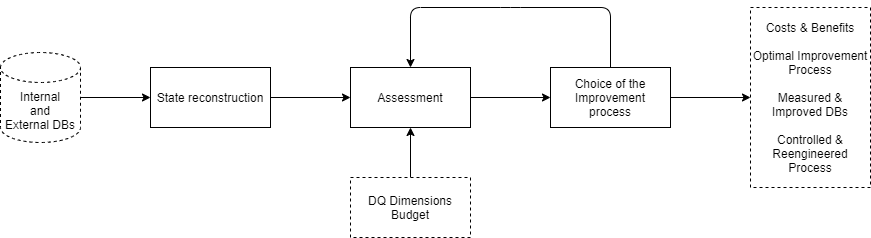
\includegraphics[width=0.9\textwidth]{figures/cdqm-diagram.png}
    \caption{Diagram of the CDQ methodology~\cite{batini2008}}
    \label{fig:cdqm-diagram}
\end{figure}
\FloatBarrier

\subsection{State reconstruction}

TODO

\subsection{Assessment}

TODO

\subsection{Choice of the optimal improvement process}

TODO

\section{BODQ}

Otto et al. (2011) developed a design process for the identification of business oriented DQ metrics~\cite{otto2011}.
The paper does not present any concrete DQ metrics even though they studied data quality problems in three companies.
Instead, those three companies' data problems were used to create an assumption that data defects cause business problems~\cite{otto2011}.
According to Otto et al. (2011), the identification of DQ metrics therefore should be based on how the data impacts process metrics~\cite{otto2011}.

A method engineering (ME) is used to design the framework.
Methodology therefore consists of five components:

\begin{itemize}
    \item design activities,
    \item design results,
    \item meta-model,
    \item roles and
    \item techniques.
\end{itemize}

\subsection{Meta-model}

Otto et al. (2011) describe entities and relations used to characterize the activities of the procedure model~\cite{otto2011}.

\begin{figure}[htb]
    \centering
    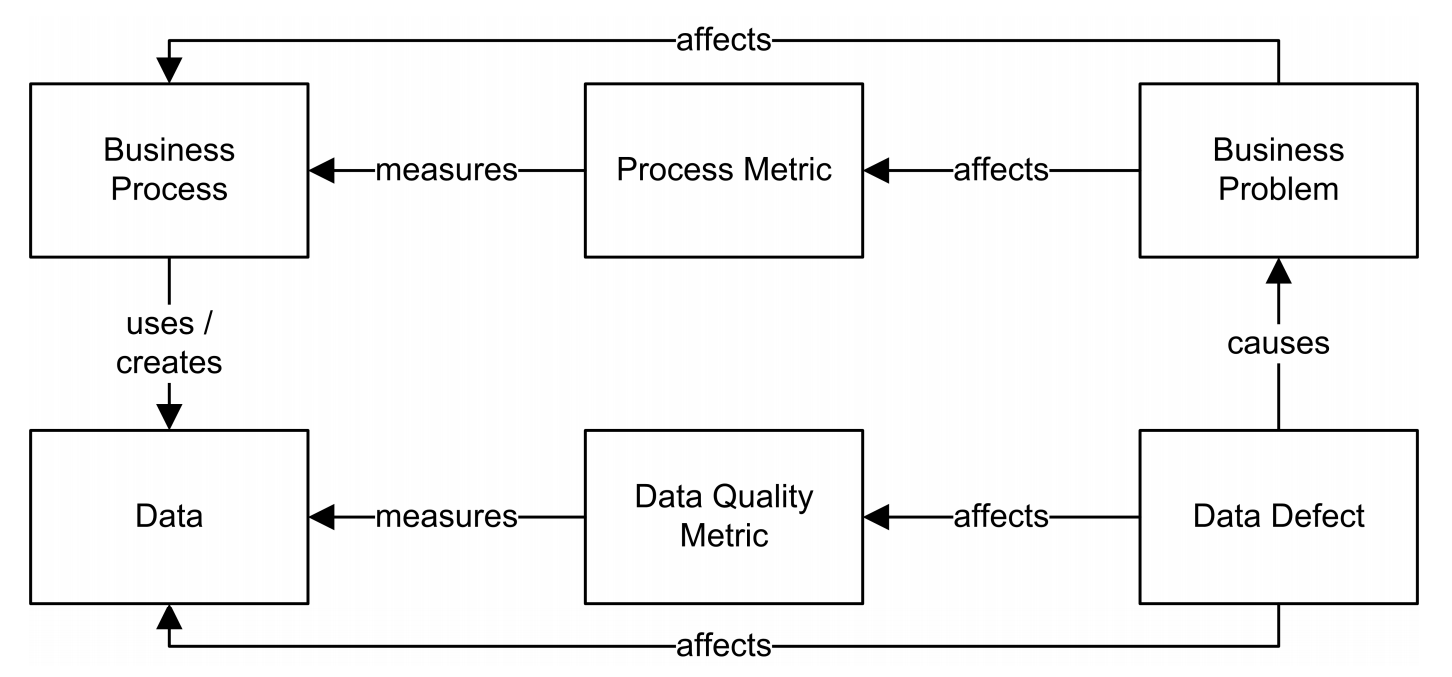
\includegraphics[width=0.9\textwidth]{figures/otto-figure-1.png}
    \caption{Entities and relations of a business oriented data quality metric~\cite{otto2011}}
    \label{fig:otto-figure-1}
\end{figure}
\FloatBarrier

\subsubsection{Business Problem}

Business problem is either system state (e.g. the package cannot be delivered) or incident (e.g. scrap parts production) causing decrease of system performance, therefore impacts \textit{process metrics} results.
It directly impacts business process and is defined by \textit{probability of occurence}\footnotemark and \textit{intensity of impact}\footnotemark.

\footnotetext[1]{Probability of occurence of event \( E \) can be denoted as \( P(E) = \frac{r}{n} \), where \( r \) is number of ways \( E \) can happen from all possible ways \( n \), \( P(E) \in [0, 1] \).}
\footnotetext[2]{
    Intensity of impact is a measure of the time-averaged power density of a wave at a particular location.
    In our case, intesity should be defined as \( I = \frac{\langle BC \rangle}{BA} \), where \( \langle BC \rangle \) is time-averaged business cost of problem and \( BA \) business area through which the problem propagates during certain time frame, \( I \in [0, \inf] \).
    If we define business area as sum of employees impacted by problem and their time spend to solve it, the unit of intensity would be costs per hour.
}

\subsubsection{Business Process}

By business process is meant sequence of tasks intended to generate value for customer and profit for the company.
The business process is controlled and defined as part of a~business strategy with corresponding modeling and measuring tools such as BPMN~2.0 or Key Performance Indicators (KPIs).

\subsubsection{Process Metric}

Quantitative measure of the degree to which a process fulfill a given quality attribute (e.g. scrap rate).

\subsubsection{Data}

Data is representation of objects and object relations.

\subsubsection{Data Defect}

It is an incident (e.g. wrong entered data), causing value decrease of data quality metrics.
As well as \textit{business problem}, a data defect poses a risk in terms of \textit{probability of occurence} and \textit{intensity of impact}.

\subsubsection{Data Quality Metric}

Quantitative measure of the degree to which data fulfill a given quality attribute (e.g. accuracy, consistency, currency,\ldots).

\subsection{Procedure Model}\label{subsec:procedure-model}

Procedure model defined by Otto et al. (2011) consists of three phases and seven activities.
Activity flow model is shown in the figure~\ref{fig:otto-figure-2}.
Letter color codes under the activities indicate degree of usage in the respective companies mentioned in the paper.
Black color means that activity was fully used, grey color means partial usage and white indicates no use at all.

\begin{figure}[htb]
    \centering
    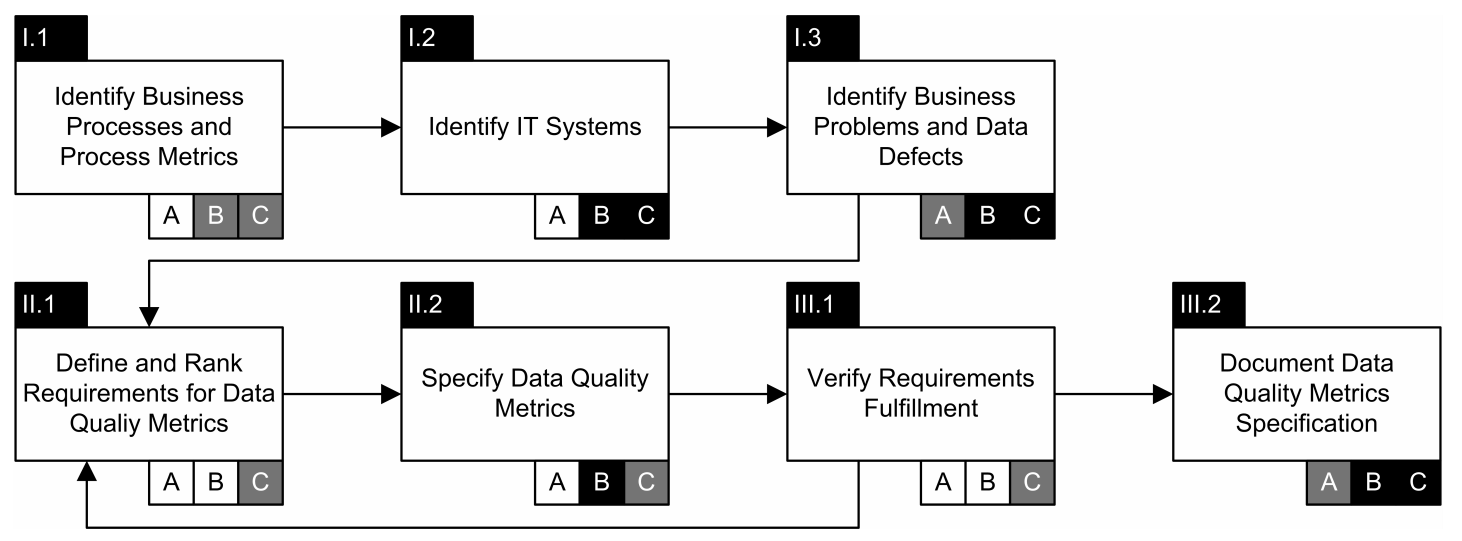
\includegraphics[width=0.9\textwidth]{figures/otto-figure-2.png}
    \caption{Procedure model and degree of usage of activities in each case~\cite{otto2011}}
    \label{fig:otto-figure-2}
\end{figure}
\FloatBarrier

\subsubsection{Phase 1}

First phase is used to collect information.
It consists of three activities:

\begin{enumerate}
    \item Identify Business Processes and Process Metrics,
    \item Identify IT Systems,
    \item Identify Business Problems and Data Defects.
\end{enumerate}

\subsubsection{Phase 2}

Second phase is used to specify requirements and design data quality mestrics.
It consists of two activities:

\begin{enumerate}
    \item Define and Rank Requirements for Data Quality Metrics,
    \item Specify Data Quality Metrics.
\end{enumerate}

\subsubsection{Phase 3}

Third phase is intended to approve and decument results.
As well assecond phase, this one consists of two activities:

\begin{enumerate}
    \item Verify Requirements Fulfillment,
    \item Document Data Quality Metrics Specification.
\end{enumerate}

\subsection{Roles}

In the last part, the authors declare six roles and their assignment to activities from section~\ref{subsec:procedure-model}.
Those roles are:

\begin{itemize}
    \item Chief Data Steward,
    \item Business Data Steward,
    \item Technical Data Steward,
    \item Process Owner,
    \item Process user and
    \item Sponsor.
\end{itemize}

\section{ORME}

Batini et al. (2007) provided DQ assessment methodology called ORME (from italian word \enquote{orme} meaning track or trace).
The methodology consists of four Data Quality Risk evaluation phases:

\begin{enumerate}
    \item prioritization,
    \item identification,
    \item measurement,
    \item monitoring.
\end{enumerate}

In the work, authors provided a comprehensive classification of costs of poor data quality.
In short, they categorized costs into three classes:

\begin{itemize}
    \item current cost of insufficient data quality,
    \item cost of IT/DQ initiative to improve current quality status,
    \item benefits gained from improvement initiative implementation.
\end{itemize}

\subsection{Prioritization}

In this phase the model reconstruction happen.
All the relationships among organization units, processes, services and data are put together and organized e.g. in the form of matrices (database/organization matrix, dataflow/organization matrix, database/process matrix).
The main goal is to provide map of the main data use across data providers, consumers and flows.

\subsection{Identification}

This phase main focus is on identification of loss events and definition of overall economic loss metrics.
In this case, loss can be expressed in 
\begin{enumerate*}[label=(\roman*)]
    \item absolute values (e.g. 100 USD),
    \item a percentage with respect to reference variables (e.g. 10\% of GDP), or
    \item a qualitative evaluation (e.g. low-medium-high).
\end{enumerate*}

\subsection{Measurement}

In this phase actual qualitative and quantitative assessment of data quality is conducted.

\subsection{Monitoring}

The last phase establishes a feedback loop and threshold in the DQ assessment process.
DQ dimensions should be, according to the authors, evaluated periodically.
Therefore quality rule violation allerts and automatic processes should be defined in order to ensure required DQ levels.

Authors suggest discriminant analysis as an easy and effective way of loss event identification.
The goal is to identify loss event based on set of new values in the data source.
The model is build on a training set, with two classes (\textit{loss} and \textit{no loss}) in consideration.
A set of linear functions from predictors is constructed,

\begin{equation*}
    L = b_1 x_1 + b_2 x_2 + \ldots + b_3 x_3 + c
\end{equation*}

where \( b_k \) are discriminant coeficient, \( x_k \) are input variables (predictors) and \( c \) is a constant.

\newpage
\section{Other}

\begin{figure}[htb]
    \centering
    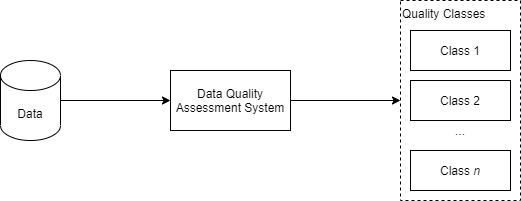
\includegraphics[width=0.9\textwidth]{figures/dq-simple.png}
    \caption{}
    \label{fig:dq-simple}
\end{figure}
\FloatBarrier

\begin{figure}[htb]
    \centering
    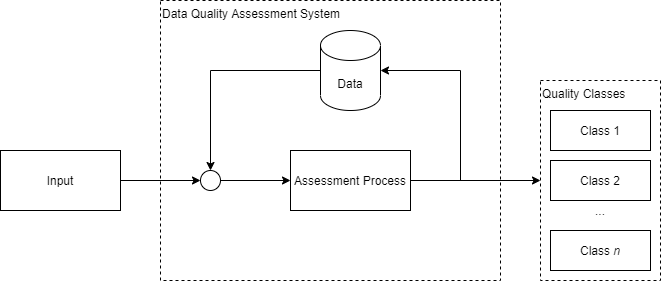
\includegraphics[width=0.9\textwidth]{figures/dq-system.png}
    \caption{}
    \label{fig:dq-system}
\end{figure}
\FloatBarrier

\section{Data Quality Attributes}

Eppler (2006) presented list of seventy of the most used data and information quality criteria explicitly defined in the literature.
They provide criterial basis for most of the DQ frameworks.
The list is shown in the figure~\ref{fig:dq-criteria}.

\begin{figure}[htb]
    \begin{multicols}{3}
        \begin{enumerate}
            \item Comprehensiveness
            \item Accuracy
            \item Clarity
            \item Applicability
            \item Conciseness
            \item Consistency
            \item Correctness
            \item Currency
            \item Convenience
            \item Timeliness
            \item Traceability
            \item Interactivity
            \item Accessibility
            \item Security
            \item Maintainability
            \item Speed
            \item Objectivity
            \item Attributability
            \item Value-added
            \item Reputation (source)
            \item Ease-of-use
            \item Precision
            \item Comprehensibility
            \item Trustworthiness\newline (source)
            \item Reliability
            \item Price 
            \item Verifiability
            \item Testability
            \item Provability
            \item Performance
            \item Ethics
            \item Privacy
            \item Helpfulness
            \item Neutrality
            \item Ease of Manipulation
            \item Validity
            \item Relevance
            \item Coherence
            \item Interpretability
            \item Completeness
            \item Learnability
            \item Exclusivity
            \item Right Amount
            \item Existence of meta information
            \item Appropriateness\newline of meta information
            \item Target group orientation
            \item Reduction of complexity
            \item Response time
            \item Believability
            \item Availability
            \item Consistent Representation
            \item Ability to represent null values
            \item Semantic Consistency
            \item Concise Representation
            \item Obtainability
            \item Stimulating
            \item Attribute granularity
            \item Flexibility
            \item Reflexivity
            \item Robustness
            \item Equivalence of redundant or distributed data
            \item Concurrency of redundant or distributed data
            \item Nonduplication
            \item Essentialness
            \item Rightness
            \item Usability
            \item Cost
            \item Ordering
            \item Browsing
            \item Error rate
        \end{enumerate}
    \end{multicols}

    \centering
    \caption{Data \& Information Quality Criteria~\cite{eppler2006}}
    \label{fig:dq-criteria}
\end{figure}
\FloatBarrier

Uniqueness
Accuracy
Consistency
Completeness
Timeliness
Currency
Format Compliance
Referential Integrity

Two main perspectives on Data Quality Management:

Broad Perspective (from the enterprise poin of view on the lifecycle of data circulating in the company)~\cite{book:dama}
Narrow Perspective (from the viewpoint of tasks to be done by data management professionals)~\cite{pres:dcam}

% \section{AI as a~tool for security breaches mitigation}\label{sec:ai-as-a-tool-for-security-breaches-mitigation}

%In the section~\ref{subsec:evasion} the principle of \textbf{model verifiability} was already mentioned.

\subsection{Parallel hybrid systems}\label{subsec:parallel-hybrid-systems}

In the paper \say{Is machine learning cybersecurity's silver bullet?} ESET's experts sort training data into three groups - malicious, clean and potentially unwanted.
They recommend not to use algorithm own output data as inputs, because any further errors are reinforced and multiplied, as the same incorrect result enters a~loop and creates more false positives or misses of malicious items.
In the next chapter ESET points out how crucial it is to achieve an equilibrium of sufficient protection from malicious items and false positives minimised to a~manageable level.
Finally, in the chapter \textit{Machine learning by ESET - The road to augur} authors let us take a~look under the hood of their ML engine called Augur.
For malicious file detection they are using two branches:
\begin{enumerate*}[label=(\roman*)]
    \item sandbox analysis followed by advanced memory analysis and behavioural features extraction (these features are later used to train ML models),
    \item ML-based branch.
\end{enumerate*}
ML-based branch consists of two methodologies:
\begin{enumerate*}[label=(\roman*)]
    \item neural networks, specifically deep learning and long short-term memory (LSTM),

    \item consolidated output of six classification algorithms.
\end{enumerate*}
While consolidating output of those six classification algorithms, two modes (setups) are used.
The first one is used for security critical environments, making algorithm more likely to mark file as malicious if most of the previous algorithms vote it as such.
The other setup is more conservative - labelling a~sample clean if at least one algorithm comes to such conclusion.

\subsection{Serial hybrid systems}\label{subsec:serial-hybrid-systems}

\begin{enumerate}[label=(\roman*)]
    \item exposure prevention (network filtering),
    \item pre-execution detection based on machine learning,
    \item runtime control proactively looking out for suspicious behavior of devices in the network (behavioral analysis based on ML),
    \item automated response such as \textit{automatic rollback} to help restore systems to their pre-attack state, system disinfection techniques or Incident of Compromise (IoC) scanning~\cite{whitepaper:kaspersky_next_generation}.
\end{enumerate}

Features are extracted from items in hard regions, to undergo ML classifiaction.
Various types of models are pre-trained with human annotated data.
Which model is selected for classification of items in region depends on several factors - extractable features, type of objects, etc.

Second topic relate to data integrity.
There is serious concern that attackers can inject data while a~model is in the training stage to alter the inference capability or add disturbance into the input samples to change model's interpretation and distort result.

Other option is to append additional component to capture and therefore filter out malicious input sample before it gets into inference stage - \textbf{adversarial sample detection}.
Simple deterministic detector could be a~deterministic comparer having some type of \textit{distance} as a~criterion.
Detectors vary greatly - forming a~group of independent models worth exploring in other papers.
% possibility to write more about detectors - the detection model may extract related information at each layer of the original model to perform detection based on the extracted information

A deformed input samples does not effect normal classification function of a~model.
\textbf{Input reconstruction} works by deforming input samples to defend against evansion attack by adding noise, de-noising, or using an automatic encoder (a type of artificial neural network)~\cite{huawei_security}.

Last but not least method is \textbf{model verification}.
In general, verification is a~discipline of software engineering with goal to assure that software fully satisfies all the expected requirements.

\textbf{Regression analysis} methods such as linear and ordinary least squares regression are ideal to detect noise and abnormalities in the data sets.
Thanks to relative directness presents those methods easy way to fight back data poisoning attack.

\textbf{Ensemble analysis} points out that usage of multiple sub-models - each one of them trained with different training data set - reduces probability of system being affected by poisoning attacks greatly.

\begin{enumerate}
    \item \textbf{Explainable data}
    As Huawei in its paper mentions, if several representative characteristics can be found at data sets and those features are carefully selected, then a~some models can be meaningfully interpretted~\cite{huawei_security}.
    Of course, data set are not usually simple enough to make such analysis.
    Moreover, AI model can grow in complexity and even with understandable data and features in the beggining, there is no guarantee that result is intereprettable in the end.

    \item \textbf{Explainable model}
    Some of the ML models (either for classification or regression) are interprettable naturaly.
    Their typical properties are \textit{linearity}, \textit{monotonicity} and \textit{interaction features} - possibility to manually add non-linearity into the model.
\end{enumerate}

\subsection{Data security}\label{subsec:data-security}

In addition to model and architecture security mechanism, we have to consider security of data sets.
Data often contains personal information of users - so called \textit{sensitive attributes}.
Such information can be in a~form of personal identifiers or quasi-identifiers.
\textit{Personal identifier} is an unique information that identifies a~user - a~birth number, bank account number and other types of personal IDs.
\textit{Quasi-identifiers} are characteristics which needs to be used in combination with others to identify an entity - examples are gender, postal code, age or nationality.

To prevent data stealing and following re-identification of users, several models exists to protect personal information of individuals in dataset.
Those privacy models are \textbf{optimal k-anonymity}, \textbf{l-diversity}, \textbf{t-closeness} and \textbf{differential privacy}.
Three general types of attack to datasets exists:
\begin{enumerate*}[label=(\roman*)]
    \item \label{itm:reident} re-identifying an individual,
    \item \label{itm:query} query whether an individual is a~member of a~dataset,
    \item \label{itm:linking} linking an individual to a~sensitive attribute.
\end{enumerate*}

\textbf{Optimal k-anonymity} protects against both cases~\ref{itm:reident} and~\ref{itm:query} by transforming quasi-identifiers so that at least \( k - 1 \) members of set are indistinguishable from each other - group based anonymization.
Identifiers are transformed by suppression (needless attributes are replaced with \textit{dummy} values) and generalization (individual values of attributes are replaced with a~broader category - e.g.\ specific age can be replaced by a~range).
As \( k \) increases risk of data exploit reduces, on the other hand data quality decreases - we are talking about a~\textit{privacy-utility} tradeoff.
Moreover, the \( k \) is limit - in order for this method to work if \( k \) is set to \( k \triangleq 10 \) then any group must contain at least \( 10 \) individuals.
The first drawback of k-anonymity is vulnerability to \textit{homogeneity attack} which works on premise of data having sensitive value identical within a~set of \( k \) records - it is enough to find the group of records, the individual belongs to, if all of them have the same sensitive value.
Second drawback is the possibility of \textit{background knowledge attack} where attacker identifies associations among one or more quasi-identifiers and reduces the set of possible values for the sensitive attribute.

Both \textbf{l-diversity} and \textbf{t-closeness} are group based anonymization techniques building on a~concept of \textbf{optimal k-anonymity}.
In addition to \textbf{optimal k-anonymity}, \textbf{T-closeness} transforms quasi-identifiers such that each group is within a~distance \( t \) of the distribution of sensitive values for the entire dataset~\cite{web:privacy-models}.
The distance is measured as the cumulative absolute difference of the distributions, as \( t \) decreases both risk of sensitive attribute disclosure and data quality decreases.
Suppose that the sensitive attribute is salary.
Each group's frequency distribution of salary will be within a~distance \( t \) from the salary frequency distribution for the entire dataset~\cite{web:privacy-models}.

\textbf{Differential privacy} and its variants (epsilon, epsilon-delta) are statistical techniques aiming to protect data against \textit{differentiated attack}.
The model guarantees that even if someone has complete information about 99 of 100 people in a~data set, they still cannot deduce the sensitive information about the final person~\cite{web:differential-privacy}.
The mechanism works by adding random noise to the aggregate data, leaving only a~trend without possibility to figure out exact values in data (e.g.\ information that \( n\% \) of users prefer some product over another).

\subsection{Data Quality Rules}

There are a number of general data quality rules one can deduce from a Feedback-Control Systems view of information systems~\cite{orr1998}.

\begin{enumerate}
    \item Unused data cannot remain correct for very long;
    \item data quality in an information system is a function of its use, not its collection;
    \item data quality will, ultimately, be no better than its most stringent use;
    \item data quality problems tend to become worse as the system ages;
    \item the less likely some data attribute (element) is to change, the more traumatic it will be when if finally does change;
    \item laws of data quality apply qually to data and metadata.
\end{enumerate}

\subsection{System Stability}

In principle, we can classify three types of system stability:

\begin{enumerate}
    \item Stable System (Absolute and Conditional stability);
    \item Marginally Stable System;
    \item Unstable System.
\end{enumerate}

\subsection{Analytics Types}

\begin{itemize}
    \item Descriptive – what happened in the past;
    \item Diagnostic – why something happened in the past;
    \item Predictive – what is most likely to happen in the future;
    \item Prescriptive – recommends actions to affect those outcomes.
\end{itemize}

\subsection{Differential Privacy}

DQ dimensions vs DQ metrics

"Confidetial/secret data will always have limited quality."

    \chapter{Methodology}\label{ch:methodology}

The proposed data quality methodology will have two major components, a model and supporting processes.
The model defines the activities, their descriptions, goals, and the order in which they must be completed in order to ensure data quality.
Support processes will then provide additional value by increasing the security and timeliness of datasets.

\section{Model}

The methodology has several important components that need to be identified or developed.
The metamodel that covers the required components is as depicted in the Figure~\ref{fig:methodology-metamodel}.
The activities within the process model have a goal to develop those components.

Overall, the methodology consists of two main processes.
The first one is \textbf{Specification Process}.
The goal of this processs is to identify and define context specific ways to measure data quality.
The second one is an \textbf{Execution Process}.
Its main goal is to \textit{collect} and \textit{verify} data with output from \textit{Specification Process} taken into account.

\begin{figure}[htb]
    \centering
    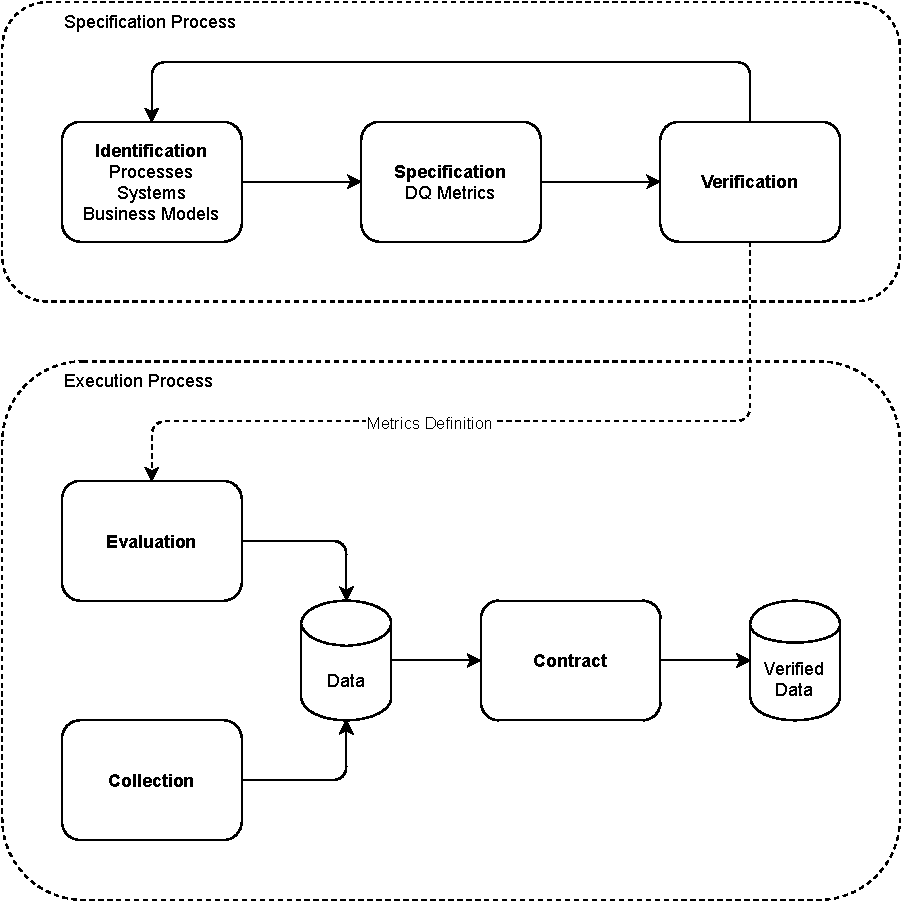
\includegraphics[width=.8\textwidth]{figures/dq-methodology.pdf}
    \caption{Methodology Metamodel}
    \label{fig:methodology-metamodel}
\end{figure}
\FloatBarrier

\subsection{Specification Process}

% Specifikační proces slouží jako nástroj pro definování kvalitativních a kvantifikovatelných požadavků na kvalitu.
The specification process serves as a tool for defining qualitative and quantifiable quality requirements.
This is a key part of the system.
% Je to však také jediná část procesu, která vyžaduje nezbytnou iniciativu analytika či analytického týmu.
However, it is also the only part of the process that requires the necessary initiative of the analyst or analytical team.
Now, we describe each part of the process.

\begin{figure}[htb]
    \centering
    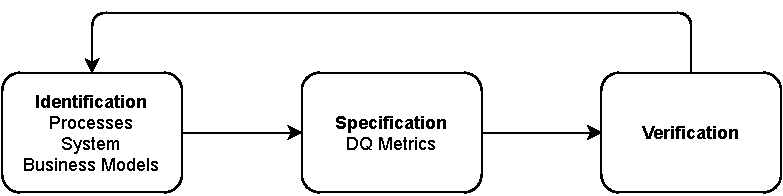
\includegraphics[width=.8\textwidth]{figures/specification-process.pdf}
    \caption{Specification Process}
    \label{fig:specification-process}
\end{figure}
\FloatBarrier

\subsubsection{Identification}

This activity focuses on identification of systems, processes and business schemes generatig data.
By identifying weak points and bottlenecks in those processes, we can find causes of poor data.
Also, we need to identify the subprocesses or activities that are mostly affected by the product data quality.

\subsubsection{Metrics Specification}

The goal of this activity is to identify the process metrics or KPIs.
Measuring data quality is all about understanding what data quality attributes are, and choosing the correct data quality metrics.
A comprehensive list of Data Quality Attributes by Eppler (2006) is available in appendix~\ref{ch:data-quality-attributes}.
Specific attributes will be further discussed in Chapter~\ref{ch:quality-classification-system}.

\subsubsection{Verification}

The last part of current process is verification.
This activity has to ensure that selected metrics are meaningful enough, capturing the actual condition of data.

\subsection{Execution Process}

The second main component is the execution process.
This includes the actual collection and validation of data against the requirements obtained by the analysis from the first process.
Ideally, in a semi-automated information system, this part runs independently, without human intervention.
However, we are aware that in many cases it is not possible to implement a fully automated system, either due to the information complexity of the task or the financial costs of system development.

\begin{figure}[htb]
    \centering
    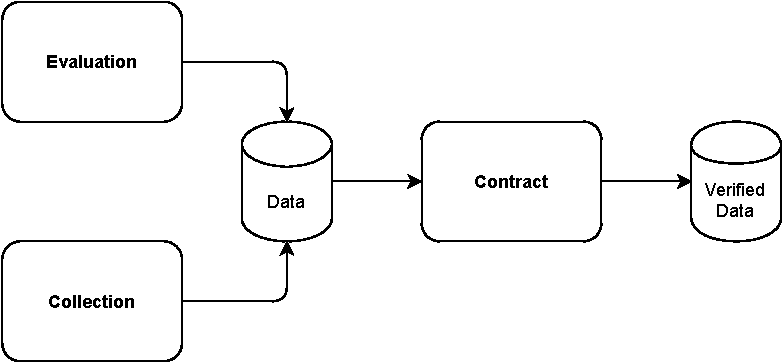
\includegraphics[width=.8\textwidth]{figures/execution-process.pdf}
    \caption{Execution Process}
    \label{fig:execution-process}
\end{figure}
\FloatBarrier

\subsubsection{Collection}

Data collection is a systematic process of gathering observations or measurements.
Data collector can be either \textit{Information System}, computer program or a human.
Before the beginning of collecting data, we need to consider:

\begin{itemize}
    \item the type of data we will collect;
    \item the methods and procedures we will use to collect, store and process data.
\end{itemize}

\subsubsection{Verification}

In our general case, verification is based on actual reliability of data, computed using DQ metrics.
In other scenarios, the verification could be based on data redundancies, therefore based on the comparison of the collected data from two or more different collectors.
If all data match, the data will be considered as valid.
If not, the data remains invalid until a further collector validates it.

Artificial Intelligence and Machine Learning could be used to further ease and optimize data verification.
Especially when processing image data and data with a high level of abstraction.

\subsubsection{Contract}

The contractual process is a subprocess that has the task of marking data as trustworthy if all the necessary requirements are met.
This is the same concept as the so-called \enquote{smart contracts}.
Smart contracts are essentially blockchain programs that are processed when mandatory conditions are fulfilled.
They are commonly used to simplify agreement implementation so that all parties can be sure of the result instantly, without intermediary intervention or time loss.
This leads to workflow automation, initiating the next step if all conditions have been satisfied.

The contracts work by following simple \enquote{if-then} statements.
This mechanism might include allocation of funds to the appropriate parties, sending notifications, or releasing a ticket.

\section{Supporting Techniques}

There are a several data quality rules one can deduce from a Feedback-Control Systems view of information systems reviewed by Orr (1998):
\begin{enumerate}
    \item unused data cannot remain correct for very long;
    \item data quality in an information system is a function of its use, not its collection;
    \item data quality cannot be better than its most strict use;
    \item data quality problems tend to become worse as the system ages;
    \item the less likely some data attribute is to change, the harder it will be to change it when the time comes;
    \item laws of data quality apply equally to data and metadata~\cite{orr1998}.
\end{enumerate}

To prevent the consequences of these rules and the unauthorized creation of data, we present two additianal concepts.
These concepts should be incorporated into the design of the information system respecting the proposed methodology.

\subsection{Proof of Constancy}

Proof of Constant Data, alias Proof of Constancy, is a way to assure a constant accuracy of data~\cite{dataeum}.
Data have to be regularly updated to keep the accuracy rate high.
Data accuracy rate will decrease progressively based on a specific time frame basis (e.g., X\% per month)~\cite{dataeum}.
This percentage is different depending on the type of data.
Datasets more sensitive to changes may see this rate decrease by 5\% to 10\% per month or day depending on the circumstances~\cite{dataeum}.
On the other hand, established, well-known sets, will see their rate decrease by 0.1\% per month or even year.
A scale of discount rates will have to be established based on the areas of interest and actual items collected.

\subsection{Proof of Trust}

Proof of Trust is an instrument for data collector evaluation~\cite{dataeum}.
The collector or generator will get \enquote*{quality score} for his/her or its collection actions~\cite{dataeum}.
The more collectors initiate, update and verify data correctly, the higher their \enquote*{quality score} will be~\cite{dataeum}.
A higher quality score leads to a higher level of \enquote*{trust}.
Incorrect collection, on the other hand, results in a retroactive decrease in the collector's quality score~\cite{dataeum}.

\section{Use Cases}

In this part, we will present several use cases to illustrate versatile use of the presented framework.

\subsection{Enterprise Information System}

Enterprises suffer from poor data quality.
We propose, following the methodology, to introduce a central register of data sources.
This central register should be supported by a set of services and a central data repository.

After a thorough analysis of data requirements and their quality, a defined set of metrics and key performance indicators parameterizes the verification chain of activities.
If the predefined quality limit is not met, the data will either be rejected or saved with an error flag.
% Jestliže data splňují požadovanou úrověň chybovosti, projdou kontraktačním procesem a jsou požadována za referenční až do doby, kdy je jejich poslední verze je nařazeným procesem kvalitativně degradována a označena za nedůvěryhodnou.
If the data meets the required level of error, they go through the contracting process and are considered as a reference until their latest version is qualitatively degraded by the ordered process (e.g., Proof of Constancy) and marked as untrusted.

% Penalizací za špatnou kvalitu by bylo automatické hlášení vyššímu managementu společnosti.
A penalty for poor quality would be automatic reporting to the company's senior management.
% Management by následně mohl uvalit na osoby zodpovědné za konkrétní datové sady a datové toky sankce ve formě snížení nebo zrušení osobních odměn.
Management could then impose sanctions on those responsible for specific datasets and data flows in the form of reductions or cancellations of personal rewards.

\subsection{IoT Cluster}

Based on the domain and usage of the IoT devices, the data repository could be either centralized (e.g., nuclear power plant cluster of secondary senzors) or decentralized (e.g., community weather stations).

The verification algorithm would - in this case - consist from two general authorities.
The first authority being \textit{k} nearest neighbours of the same sensors (or IoT devices in general), and the second one being the set of domain rules.
Nearest neighbors provide redundancy by which data can be verified.
And, of course, the data itself must meet the criteria restrictions set by the domain of use.

% Špatná kvalita by vedla ke snížení významnosti senzoru v klusteru, případně jeho dočasnému nebo úplnému vyřazení z provozu.
Poor quality would reduce the importance of the sensor in the cluster, or its temporary or complete decommissioning.
% Tento systém by vytořil i velice účinnou obranou bariéru proti útokům.
This system would also create a very effective defense barrier against attacks, especially against data poisoning.

Data poisoning is a class of attacks on machine learning algorithm where an adversary alters a fraction of the training data in order to impair the intended function of the system.
Objective can be to degrade the overall accuracy of the trained classifier, escaping security detection or to favor one product over the another.
Machine Learning systems are usually retrained after deployment to adapt to changes in input distribution, so data poisoning represents serious danger.

Qualitative degradation of data by Proof of Constancy would not be the so important, because we expect very high update frequency.
However, lower update frequancy of IoT device would suggest an error within a system, which could serve as a warning to network operators about a faulty device.
Data from defective equipment should also not be taken into account in many cases.

\subsection{Open Data Library}

The final use case demonstrates the use of a completely decentralized solution.
The system would reward those who collect and generate data, and the data would be available for use in a decentralized marketplace.
The decentralized network would democratize data access while rewarding data creators~\cite{dataeum}.

Data would be collected using an application (system) that would be used by a~community of collectors who would be rewarded for their efforts.
The reward should be determined by a~\enquote*{collection value}.

The collection value would be calculated using an algorithm that considers a number of factors, including:
\begin{itemize}
    \item demand and rarity,
    \item availability and accessibility,
    \item data licensing and
    \item market value~\cite{dataeum}.
\end{itemize}

To maintain a high level of dependability, each collector receives a quality score.
The verified data is then made available (via contract) on the decentralized marketplace and is updated on a regular basis to ensure its accuracy.

Automation of the verification process is nearly impossible due to the variety of open data.
The data must be manually verified.
As a result, a collector serves two purposes:
\begin{itemize}
    \item initiate the data collection (input and update data),
    \item verify the collected data (check a collected data not yet verified)~\cite{dataeum}.
\end{itemize}

The process guarantees that the reward for data collection is split equally between the collector and the verifier~\cite{dataeum}.
For example, the collector who initiated the data collection would receive 60-80\% of the reward~\cite{dataeum}.
The remaining 20-40\% would be obtained by the verifier~\cite{dataeum}.

Depending on the data, a decentralized network like filecoin could be used as data storage.
The use of blockchain renders the data unalterable, ensuring the transparency and traceability of the validation process (collection, verification, update).
The blockchain (which is tamper-proof, immutable, and decentralized) ensures the integrity and verification of the data on the marketplace.
This gives data users confidence and security.
The use of \textbf{Smart Contract} technology also ensures the collectors' rewards.

    \chapter{Quality Classification System}\label{ch:quality-classification-system}

The original idea was to leverage some Machine Learning classification algorithm to automatically classify datasets.
During thesis elaboration the referential materials turned out to be insufficient in providing usefull information on the topic, hence different technique was chosen (composite statistical score-card evaluation).
Shortcoming of white-papers about Machine Learning supported DQ classification probably results from the absence of well-defined general DQA algorithm and output classes.
Complexity of developing all-embracing method for DQA competes with unfolding general artificial intelligence, indeed.

Resulting system should be similar to machine learning ensemble methods (ensemble voting).

\section{Data Quality Criteria}

Tabular vs relational data
Tabular data structures: Cross-Sectional, Time-Series, Pooled Cross-Sections, Panel (Longitudal)
Metrics usability with raw (non-aggregated) and aggregated data.


In order to provide 

\subsection{Accuracy}

TODO

\subsection{Completeness}

Blake and Mangiameli (2011) defined completeness as follows.
On the level of data values, a~data value is incomplete (i.e., the metric value is zero) if and only if it is \enquote*{NULL}, otherwise it is complete (i.e., the metric value is one).
A tuple in a relation is defined as complete if all data values are complete (i.e., none of its data values is \enquote*{NULL}).
For a relation \( R \), let \( T_R \) be the number of tuples in \( R \) which have at least one \enquote*{NULL}-value and let \( N_R \) be the total number of tuples in \( R \). Then, the completeness \( C \) of \( R \) is defined as follows~\cite{blake2011}.

\begin{equation}
    C = 1 - \frac{T_R}{N_R} = \frac{N_R - T_R}{N_R}
\end{equation}

This definition of \textit{completeness} meets the requirements for metrics according to Heinrich et al. (2018).
The metric values are within the bounded interval \( \left[0; 1\right] \) for all aggregation levels.
The minimum value represents perfectly poor data quality and vice versa.
To archieve full score, no tuple must not contain a null value, as well as relations must not contain any tuple with data values which equal \enquote*{NULL}.

The metric is reliable because all configuration parameters of the metric can be determined by a database query.
Due to the existence of a mathematical formula, the metric is objective and because the metric quantifies a dimension at all quality levels according to the corresponding definition, the determination of the metric value is also valid.
The metric formula is applicable to single data values as well as to sets of data values.

\subsection{Consistency}

There are several forms of data consistency.
The \textbf{first form} is actual wide or narrow distribution of data.
In this way, consistency of data can be viewed as \textit{stability}, \textit{uniformity} or \textit{constancy}.
Typical measures include statistics such as the \textit{range} (i.e., the largest value minus the smallest value among a distribution of data), the \textit{variance} (i.e., the sum of the squared deviations of each value in a distribution from the mean value in a distribution divided by the number of values in a distribution) and the \textit{standard deviation} (i.e., the square root of the variance).

\begin{figure}[htb]
    \centering
    
    \begin{equation*}
        \sigma = \sqrt{\frac{1}{N}\sum_{i=1}^{N} (x_{i} - \mu)^2}
    \end{equation*}

    \caption{Population Standard Deviation formula}
    \label{form:population-standard-dev}
\end{figure}
\FloatBarrier

\begin{figure}[htb]
    \centering
    
    \begin{equation*}
        s = \sqrt{\frac{1}{N - 1}\sum_{i=1}^{N} (x_{i} - \bar{x})^2}
    \end{equation*}

    \caption{Sample Standard Deviation formula}
    \label{form:sample-standard-dev}
\end{figure}
\FloatBarrier

If one is evaluating the consistency of data drawn in a sample from a population, the \textit{standard error of the mean} (i.e., the standard deviation of the sampled population divided by the square root of the sample size) is often examined.
Finally, the constancy of data produced by instruments and tests is typically measured by estimating the reliability of~obtained scores.
Reliability estimates include test-retest coefficients, split-half measures and Kuder-Richardson Formula \textnumero 20 indexes~\cite{quora:consistency2017}.
For Time Series data, stationary analysis can be done.
If the data is non-stationary then it is likely to have some degree of inconsistency.

\begin{figure}[htb]
    \centering
    
    \begin{equation*}
        \sigma_{\bar{x}} = \frac{\sigma}{\sqrt{n}}
    \end{equation*}

    \caption{Standard Error of the Mean formula}
    \label{form:sem}
\end{figure}
\FloatBarrier

Then, there is \textbf{second form} of data consistency; whether data are uniformly defined throughout the dataset, that is, across variables and over time.
For example, suppose we want to use the data to estimate real estate sales per year to see how that number has changed over time.
In this case, we have to make sure the estimates of real estate sales are uniformly defined over time.
Specifically, does the data series always either include apartments or exclude apartments from the counts?
Does it always either include houses or exclude houses from the counts?
If the data sometimes include apartments, but not always, or if the data sometimes include houses, but not always, then the data are inconsistent.

The \textbf{third form} of consistency tightly coupled with relational databases and their referential integrity.
A relational database is said to be ACID (vs non-relational BASE), meaning
\begin{enumerate*}[label=(\roman*)]
    \item atomicity,
    \item consistency,
    \item isolation and
    \item durability.
\end{enumerate*}
The term onsistency there refers to the requirement that any given database transaction must affect data only in allowed ways, therefore data must be valid according to all defined rules, including constraints, cascades, triggers, and any combination thereof.

Inconsistencies in data can be due to changes over time and/or across variables for example, in
\begin{enumerate*}[label=(\roman*)]
    \item vintages or time periods,
    \item units,
    \item levels of accuracy,
    \item levels of completeness,
    \item inclusions and exclusions.
\end{enumerate*}
Those inconsistencies occur most often when merging or aggregating datasets, therefore the user has to make sure data are consistently defined throughout.

\subsection{Timeliness}

Timeliness is another one of the major dimensions in the field of data quality.
Obsolete data suppress innovation, therefore businesses and startups want to trust the data publisher that the data will remain available and relevant, especially when using open data or reference data from central registers.
A measure of timeliness has to focus on the update cycle.
Automation must be a key part of this process, leading to the efficiency in publishing and processing of data.
Meeting all these points is a necessary, but not sufficient condition to create a sustainable data ecosystem.

Atz (2014) proposed an unique metric for measuring the timeliness of data.
The research defines timely dataset as a product of function of the forecast update frequency (a dataset released annualy will be updated only once a year)~\cite{atz2014tau}.
The concept of timeliness \( T \) can be expressed by the equation~\ref{eq:timeliness}.

\begin{equation}\label{eq:timeliness}
    T = I \frac{f_U}{today - last update}
\end{equation}

In the equation~\ref{eq:timeliness}, the \( I \) is an indicator function causing \textit{Heaviside} step function effect returning 1 when the ratio is greater than one and 0 otherwise.
For example, a dataset with a daily cycle and a last major update last month would result in a 0.
On the other hand, a dataset with monthly cycle and an update in last two weeks, would yield 1.
In the equation \( f_U \) represents \textit{update frequency}; the terms \textit{today} and \textit{last update} are timepoints corresponding to the names.

% Důvod přítomnosti indikátorové funkce je ten, že nemáme nástroj, kterým bychom zhodnotili způsob stárnutí datasetu.
The reason for the presence of the indicator function is that we do not have a tool to evaluate the aging of the dataset.
% Data mohou zastarávat lineárně a spojitě, ale také nelineárně a nespojitě.
Data can become obsolete linearly and continuously, but also non-linearly and discontinuously.
% Tato funkční závislost je nám skryta, data považujeme tedy buď za aktuální nebo zastaralá.
This functional dependence is hidden from us, so we consider the data to be either current or obsolete.

% \[ T = \begin{cases} 0 & x\leq 0 \\ \frac{100-x}{100} & 0\leq x\leq 100 \\ 0 & 100\leq x \end{cases} \]

Atz (2014) introduced a metric for measuring data catalogue timeliness, \( \tau \).
In general, minor changes such as typo correction should not be considered as an update.

\begin{equation*}
    \tau = \frac{1}{N} \sum_{i = 1}^N I \left( \frac{f_{U_i} \cdot \lambda + \delta}{today - {last update}_i} \right)
\end{equation*}

The \( \tau \) of a data catalogue is the average across datasets, indicated by the subscript \textit{i}~\cite{atz2014tau}.
The number of datasets in the catalog is denoted by the \textit{N}.

Two parameters in a linear form have been introduced to the core of the expression.
The lambda (\( \lambda \)) is degree of freedom relative to the update frequency; the days we allow the update of the data catalog.
For example, considering 5\% of the time reserve (e.g., due to ETL delays), the annual renewal dataset is going have a buffer of 0.6 months and for a monthly dataset it implies 1.5 days in tolerance.
The delta (\( \delta \)) is a fixed number of days applicable to all datasets, for example one day for processing~\cite{atz2014tau}.

\begin{table}[htbp]
    \centering

    \begin{tabular}{@{}ll@{}}
        \toprule
        \( \tau \)  & Data Timeliness   \\ \midrule
        0.9-1       & exemplar          \\
        0.7-0.9     & standard          \\
        0.5-0.7     & ok                \\
        0.25-0.5    & poor              \\
        0-0.25      & obsolete          \\
        \bottomrule
    \end{tabular}

    \caption{Proposed benchmarks for different levels of \( \tau \)~\cite{atz2014tau}}
    \label{table:timeliness-benchmarks}
\end{table}
\FloatBarrier

    \newenvironment{QandA}{\begin{enumerate}[label=\bfseries\alph*.]\bfseries}
        {\end{enumerate}}
\newenvironment{answered}{\par\normalfont}{}

\chapter{Case Study}\label{ch:case-study}

In December 2019, a virus known as COVID-19 was first identified in Wuhan, China~\cite{seznam-korona2021}.
Three months later, on March 1, 2020, the first three cases of the disease were confirmed in the Czech Republic~\cite{seznam-korona2021}.
The disease has shown and continues to show the shortcomings of social and political environment worldwide.
But the disease, although very serious, has given us many opportunities.
One such opportunity is open datasets made available by state institutions.

In the following part of the work we will try to analyze the state of datasets provided by the institutions of the Czech Republic.
We apply the metrics defined in Chapter 3 to the data in order to objectively measure their quality and comment on the results.
Available datasets as of April 1, 2020 from the URL address \url{https://onemocneni-aktualne.mzcr.cz/} are listed in Appendix~\ref{ch:dataset-collection}.

\section{Technical Analysis}

The data can be downloaded via the REST API in JSON, in addition, the data can be downloaded in CSV together with metadata also in JSON format.
The format of the JSON data file can be seen in Figure~\ref{ls:data}.
All data files contain one main object, with three keys (modified, source and data).
The \enquote{modified} key contains the date of the dataset update in ISO 8601 format with the time offset from UTC (Coordinated Universal Time).
The \enquote{source} key contains the URL of the dataset, especially the protocol and domain name.
The last key, the data, contains an array of json objects with a structure given by the metadata.
This is an array of objects even if the array contains only one object.

\begin{figure}[htb]
    \centering

    \begin{lstlisting}[language=json,firstnumber=1]
{
    "modified": "2021-04-18T12:28:42+02:00",
    "source": "https:\/\/onemocneni-aktualne.mzcr.cz\/",
    "data": [
        {
            ...
        }
    ]
}
    \end{lstlisting}

    \caption{Data file structure}
    \label{ls:data}
\end{figure}
\FloatBarrier

An example of the structure of the metadata file can be found in the appendix~\ref{ch:metadata-file-structure}.

\section{Data Quality Analysis}

Long et al. (2004) wrote a comprehesive data quality checklist for emergency medical services data~\cite{long2004}.
We will use this checklist as a base for our own data evaluation.

\subsection{Relevance}

\begin{table}[htbp]
    \centering

    %\begin{tabular}{@{}llrrrrrrrrrr@{}}
    \begin{tabular}{llrrrrrrrrrr}
        \toprule
        \multirow{2}{*}{Dimension}  & \multirow{2}{*}{Characteristics}  & \multicolumn{10}{c}{Criteria}         \\ \cmidrule(lr){3-12}
                                    &                                   & a & b & c & d & e & f & g & h & i & j \\ \midrule
        \multirow{2}{*}{Relevance}  & Adaptability                      & 2 & 2 & 2 & 0 & 2 & 0 & 2 & 0 & 2 &   \\
                                    & Value                             & 2 & 0 &   &   &   &   &   &   &   &   \\
        \bottomrule
    \end{tabular}

    \caption{Evaluation of criteria for dimension Relevance}
    \label{table:relevance-benchmark}
\end{table}
\FloatBarrier

\subsubsection{Value}

\begin{QandA}
    \item The purpose of the data is clear.
    \begin{answered}
        Yes, the general purpose of the data is obvious.
        The data is provided by the Institute of Health Information and Statistics of the Czech Republic (IHIS CR).
        Individual datasets have a description that specifies their purpose.
    \end{answered}

    \item The data shed light on the issues of most importance to users and the data are used in policy formulation and decision making.
    \begin{answered}
        Yes, the data provide information on the current development of the epidemic situation in the Czech Republic.
        The dynamics of the \textit{Compartmental Model} can be derived from the data and thus predictive analysis can be done.
        The data are used for policy formulation and decision making.
    \end{answered}

    \item There are no other more valid sources for the data.
    \begin{answered}
        Yes, the data is provided by a government agency.
        There is no other source of data for the public.
    \end{answered}

    \item Client liaison mechanisms are in place and client needs are monitored.
    \begin{answered}
        Unknown.
    \end{answered}

    \item How the data are used is known and well understood.
    \begin{answered}
        The Institute of Health Information and Statistics of the Czech Republic publishes summaries of the epidemiological situation and other reports, including descriptions of methodologies for using data for predictions.
        Formally, this point is met.
    \end{answered}

    \item Client evaluations are conducted and reviewed.
    \begin{answered}
        Unknown.
    \end{answered}

    \item The data are found to meet the needs of its users.
    \begin{answered}
        In this case, as \enquote{needs of the users} is considered the awareness of the general public.
        From this point of view, the question is met.
    \end{answered}

    \item Client evaluations are conducted and reviewed.
    \begin{answered}
        During the publication of datasets, many modifications and additions were made.
        Feedback taken into account.
        However, we do not have information to what extent.
        The point is therefore classified as \textbf{unknown}.
    \end{answered}

    \item The data are found to be worth the resources dedicated to its production.
    \begin{answered}
        Yes, these data are necessary to inform the public about the current state of development of the pandemic.
        Almost any expenditure is worthwhile in this case.
    \end{answered}

\end{QandA}

\subsubsection{Adaptability}

\begin{QandA}
    \item The data can be used to inform emerging issues and can adapt to change.
    \begin{answered}
        Yes, this has been demonstrated in the past by the introduction of anti-epidemic measures and the changes that have been introduced in the datasets.
    \end{answered}

    \item Ongoing explicit program review and priority determination are conducted.
    \begin{answered}
        The degree of review by the data issuer is \textbf{unknown}.
    \end{answered}

\end{QandA}

\subsection{Accuracy}

\begin{table}[htbp]
    \centering

    %\begin{tabular}{@{}llrrrrrrrrrr@{}}
    \begin{tabular}{llrrrrrrrrrr}
        \toprule
        \multirow{2}{*}{Dimension}  & \multirow{2}{*}{Characteristics}  & \multicolumn{10}{c}{Criteria}         \\ \cmidrule(lr){3-12}
                                    &                                   & a & b & c & d & e & f & g & h & i & j \\ \midrule
        \multirow{13}{*}{Accuracy}  & Form Design and Completion        & 2 & 2 & 2 & 1 & 0 & 0 & 0 & 1 & 1 & 0 \\
                                    & Frame                             & 2 & 2 &   &   &   &   &   &   &   &   \\
                                    & Over Coverage                     & 0 & 0 &   &   &   &   &   &   &   &   \\
                                    & Under Coverage                    & 0 & 1 &   &   &   &   &   &   &   &   \\
                                    & Response                          & 1 & 2 &   &   &   &   &   &   &   &   \\
                                    & Completeness                      & 0 & 0 & 0 & 0 &   &   &   &   &   &   \\
                                    & Bias                              & 0 & 1 & 0 & 0 & 0 & 0 &   &   &   &   \\
                                    & Validity                          & 2 & 0 & 0 & 1 &   &   &   &   &   &   \\
                                    & Reliability                       & 0 & 1 & 0 &   &   &   &   &   &   &   \\
                                    & Collection                        & 2 & 0 & 2 & 0 & 0 & 0 & 1 & 2 & 1 & 1 \\
                                    & Processing                        & 0 & 0 & 1 & 0 &   &   &   &   &   &   \\
                                    & Imputation                        & 0 & 2 &   &   &   &   &   &   &   &   \\
                                    & Analysis                          & 0 & 0 & 0 & 1 &   &   &   &   &   &   \\
        \bottomrule
    \end{tabular}

    \caption{Evaluation of criteria for dimension Accuracy}
    \label{table:accuracy-benchmark}
\end{table}
\FloatBarrier

\subsubsection{Form Design and Completion}

\begin{QandA}
    \item The data retrieval form was designed by a team that includes methodologists, a form design expert, representatives for those who are responsible for completing the form, as well as other subject matter experts.
    \begin{answered}
        Data are issued by IHIS CR.
        The criterion is \textbf{met}.
    \end{answered}

    \item The purpose and population of interest are clear and well documented.
    \begin{answered}
        The purpose of the data is clear.
        The population to be monitored is precisely defined, individuals infected with COVID-19 and individuals tested or vaccinated.
    \end{answered}

    \item There is adequate justification for each field gathered.
    \begin{answered}
        The accessible data is preprocessed and therefore each field in the dataset has a purpose.
        The purpose may not be obvious at first glance, but all fields are defined and annotated in the metadata. 
        We consider this criterion to be \textbf{met}.
    \end{answered}

    \item The form is user-friendly and is accompanied by a clear, readily accessible, and user-friendly manual that describes in detail the data collection guidelines including when and how to complete the form and defines each field in detail.
    \begin{answered}
        Data is available through a well-defined API.
        Although instructions for data collection are either missing or very difficult to find.
        As this absolutely essential requirement is violated, we consider the criterion to be \textbf{not met}.
    \end{answered}

    \item Those responsible for completing the form receive training so that they are able to properly complete the form.
    \begin{answered}
        Unknown.
    \end{answered}

    \item As part of training, the importance of the data is conveyed and those responsible for completing the form are tested and immediate feedback is provided regarding the reliability and validity of their performance.
    \begin{answered}
        Unknown.
    \end{answered}

    \item Those responsible for completing the form are allocated the time and have the motivation to do so, as well as confidence in the form completion process.
    \begin{answered}
        Unknown.
    \end{answered}

    \item The data are monitored for outliers, logical errors, completeness, and consistency and ongoing monitoring and constructive feedback is provided to the primary collectors where necessary.
    \begin{answered}
        Data monitoring information is unknown. But the data contains logical errors.
        Feedback to primary collectors (hospitals, medical facilities and sanitation stations) is very difficult to implement.
        We consider the criterion to be \textbf{not met}.
    \end{answered}

    \item Any major revisions to the original form design (purpose, structure, etc.) of the database and the dates of any major revisions are known, documented, and readily available. Moreover, an explicit consideration of overall trade-offs between accuracy, cost, timeliness, and respondent burden was conducted at the design stage.
    \begin{answered}
        Information on the design phase is unknown.
        To our knowledge, changes to the API design are not available to the public, if documented at all.
        For this reason, we consider the criterion to be \textbf{not met}.
    \end{answered}

    \item A revised form is pilot tested until high standards of reliability and validity are met and the pilot test results are readily available.
    \begin{answered}
        Unknown.
    \end{answered}

\end{QandA}

\subsubsection{Frame}

By the "frame" we mean the structure of files containing data.
The COVID-19 API is well documented and easy to understand.
During the epidemic, the API was shown to be continuously updated.

\begin{QandA}
    \item The frame is known and documented.
    \begin{answered}
        The criterion is \textbf{met}.
    \end{answered}

    \item The frame is maintained in an ongoing manner.
    \begin{answered}
        The criterion is \textbf{met}.
    \end{answered}

\end{QandA}

\subsubsection{Over Coverage}

Over-coverage is caused by the existence of objects not belonging to the frame, as well as units that appear in the target population multiple times~\cite{over-coverage}.

\begin{QandA}
    \item Only qualifying data suppliers are on the frame.
    \begin{answered}
        Information on data suppliers is not available.
        The criterion is \textbf{unknown}.
    \end{answered}

    \item The data are checked for duplicates and erroneous entries from qualifying suppliers.
    \begin{answered}
        Unknown.
    \end{answered}

\end{QandA}

\subsubsection{Under Coverage}

Over-coverage is caused by exclussion of objects belonging to the frame~\cite{under-coverage}.

\begin{QandA}
    \item Data are received from all qualifying data suppliers on the frame.
    \begin{answered}
        Unknown.
    \end{answered}

    \item The list of those actually sending data are compared to independent lists.
    \begin{answered}
        Given the nature of the data, the existence of third party lists can be questioned.
        We therefore consider the criterion not to be met.
    \end{answered}

\end{QandA}

\subsubsection{Response}

\begin{QandA}
    \item The overall expected and actually received number of records are known and tracked per year and response across month is checked and compared against previous years.
    \begin{answered}
        This criterion is in principle difficult to meet.
        The number of records is not known in advance and, due to the relatively short existence of the dataset, it was not possible until recently to compare the data with previous time periods.
        We consider the criterion to be \textbf{not met}, although the question remains whether it is valid for our case.
    \end{answered}

    \item The amount of missing data per record is known and tracked per field per year and key fields (e.g., age, gender, and clinical code) are at least 98\% complete.
    \begin{answered}
        Key data has been remeasured, the criterion is \textbf{met}.
    \end{answered}

\end{QandA}

\subsubsection{Completeness}

\begin{QandA}
    \item The patient service form/chart used for data retrieval from abstraction is easy to understand.
    \begin{answered}
        Information on internal procedures is \textbf{not known}.
    \end{answered}

    \item The form/chart used for abstraction is complete.
    \begin{answered}
        Information on internal procedures is \textbf{not known}.
    \end{answered}

    \item All patient encounters/visits are abstracted and represented in the database.
    \begin{answered}
        Information on internal procedures is \textbf{not known}.
    \end{answered}

    \item All fields are systematically completed per patient record.
    \begin{answered}
        Information on internal procedures is \textbf{not known}.
    \end{answered}

\end{QandA}

\subsubsection{Bias}

\begin{QandA}
    \item Explicit standard guidelines are in place and adherence is monitored for data collection
    \begin{answered}
        Information on internal procedures is \textbf{not known}.
    \end{answered}

    \item Clear guidelines and training eliminate as much as possible the need for interpretation.
    \begin{answered}
        The IHIS CR does not provide data training for external candidates and we do not have information available about the training of internal employees.
        The data are quite clear, but due to their sensitivity it is appropriate to interpret them.
        For this reason, we consider the criterion to be \textbf{not met}.
    \end{answered}

    \item For data that need to be classified, clear coding standards are available.
    \begin{answered}
        Information on internal procedures is \textbf{not known}.
    \end{answered}

    \item For data that need to be classified, the available standards are adhered to.
    \begin{answered}
        Information on internal procedures is \textbf{not known}.
    \end{answered}

    \item For data that need to be classified, only highly trained certified staff classify the data.
    \begin{answered}
        Information on internal procedures is \textbf{not known}.
    \end{answered}

    \item Sources of bias (e.g., upcoding) are understood and eliminated if possible and ongoing quality assurance tests ensure that data collection, abstraction, and entry are conducted in a standard manner according to guidelines.
    \begin{answered}
        Information on internal procedures is \textbf{not known}.
    \end{answered}

\end{QandA}

\subsubsection{Validity}

\begin{QandA}
    \item The patient service form/chart is complete and reflects the patient encounter and the codesheet or abstract that is based on the form/chart reflects what is in the form/chart.
    \begin{answered}
        Since we do not work with complete input data, this question is irrelevant.
        However, we have a dataset with patient data (age, gender, residence) that directly corresponds to the input data.
        For this reason, we consider the requirement to be \textbf{met}.
    \end{answered}

    \item Adequate resources are in place to ensure valid timely data and ongoing database improvement.
    \begin{answered}
        Information on internal procedures is \textbf{not known}.
    \end{answered}

    \item Random audits and/or reabstraction studies are conducted and the data are compared to external sources of the same or similar data (if possible).
    \begin{answered}
        Information on internal procedures is \textbf{not known}.
    \end{answered}

    \item Validity coefficients are available and are greater than or equal to 0.8 for key data elements (i.e., postal code, patient age, most responsible diagnosis, procedures, and comorbities).
    \begin{answered}
        The IHIS CR itself does not provide any validity metrics.
        This requirement is \textbf{not met}.
    \end{answered}

\end{QandA}

\subsubsection{Reliability}

\begin{QandA}
    \item Reliability studies of key data elements (e.g., age, gender, and clinical code) are conducted at regular intervals.
    \begin{answered}
        Information on internal procedures is \textbf{not known}.
    \end{answered}

    \item Intra rater coefficients are available.
    \begin{answered}
        The IHIS CR itself does not provide any reliability metrics.
        This requirement is \textbf{not met}.
    \end{answered}

    \item Rater coefficients are greater than or equal to 0.8 for key data elements (i.e., postal code, patient age, most responsible diagnosis, procedures, and comorbities).
    \begin{answered}
        Intra-rater coefficients are not available.
        The criterion is \textbf{not known}.
    \end{answered}

\end{QandA}

\subsubsection{Collection}

\begin{QandA}
    \item Standard data retrieval form is in place.
    \begin{answered}
        From the data user's point of view, the data is accessible in standard formats.
        This requirement is \textbf{met}.
    \end{answered}

    \item Range checks are place for all fields at data entry and key logic checks are run (e.g., checks for clinical impossibilities or date of birth greater than call date).
    \begin{answered}
        Information on internal procedures is \textbf{not known}.
    \end{answered}

    \item Standard data specifications are provided to vendor(s).
    \begin{answered}
        The institute provides a dictionary with metadata.
        This requirement is \textbf{met}.
    \end{answered}

    \item Standard test data are used to test edits.
    \begin{answered}
        Information on internal procedures is \textbf{not known}.
    \end{answered}

    \item Data entry software and equipment are user friendly.
    \begin{answered}
        Information on internal software and hardware is \textbf{not known}.
    \end{answered}

    \item Staff is available and motivated to enter the data and data entry is monitored and constructive feedback is provide to staff.
    \begin{answered}
        Information on internal procedures is \textbf{not known}.
    \end{answered}

    \item Edit errors are set aside and made available for analysis.
    \begin{answered}
        The institute does not provide any dataset regarding data errors.
        This requirement is \textbf{not met}.
    \end{answered}

    \item Data entry of abstracted data takes place in close proximity to the original data (original forms/charts).
    \begin{answered}
        Although no information is available about internal processes, the data is prone to factual accuracy.
        Let us consider this requirement to be \textbf{met}.
    \end{answered}

    \item Error detection reports are generated.
    \begin{answered}
        The institute does not provide any documentation regarding data errors.
        This requirement is \textbf{not met}.
    \end{answered}

    \item Error correction is documented.
    \begin{answered}
        The institute does not provide any documentation regarding data errors.
        This requirement is \textbf{not met}.
    \end{answered}

\end{QandA}

\subsubsection{Processing}

\begin{QandA}
    \item All programming is tested and the results are documented.
    \begin{answered}
        Information on internal procedures is \textbf{not known}.
    \end{answered}

    \item Ongoing quality control checks are conducted on electronically extracted data.
    \begin{answered}
        Information on internal procedures is \textbf{not known}.
    \end{answered}

    \item Documentation on how the various systems involved interact, extract, change, and/or append the data exists and is available.
    \begin{answered}
        The information mentioned in the request is not known to the public.
        This requirement is \textbf{not met}.
    \end{answered}

    \item Ongoing tests are run to ensure all systems are interacting properly.
    \begin{answered}
        Information on internal procedures is \textbf{not known}.
    \end{answered}

\end{QandA}

\subsubsection{Imputation}

The replacement of approximate values for incomplete or conflicting data elements is known as data imputation~\cite{data-imputation}.
The substituted values are meant to produce a data record that is not subject to edit failure~\cite{data-imputation}.

\begin{QandA}
    \item Imputation is automatically derived.
    \begin{answered}
        Information on internal procedures is \textbf{not known}.
    \end{answered}

    \item The raw data are preserved.
    \begin{answered}
        Although information on internal processes is not available, it can be assumed with great certainty that the original data is not modified in any way.
        Let us consider this requirement to be \textbf{met}.
    \end{answered}

\end{QandA}

\subsubsection{Analysis}

\begin{QandA}
    \item Edit errors are analyzed.
    \begin{answered}
        Information on internal procedures is \textbf{not known}.
    \end{answered}

    \item Error detection analyses are conducted and the data are checked for missing data.
    \begin{answered}
        Information on internal procedures is \textbf{not known}.
    \end{answered}

    \item Outliers or other suspicious data are investigated.
    \begin{answered}
        Information on internal procedures is \textbf{not known}.
    \end{answered}

    \item Regular standard summary analyses are conducted and made available.
    \begin{answered}
        Although we have summary data in the form of a graphical report, it is not a statistical report summarizing the qualitative status of the data.
        For this reason, we consider the requirement to be \textbf{not met}.
    \end{answered}

\end{QandA}

\subsection{Timeliness}

\begin{table}[htbp]
    \centering

    %\begin{tabular}{@{}llrrrrrrrrrr@{}}
    \begin{tabular}{llrrrrrrrrrr}
        \toprule
        \multirow{2}{*}{Dimension}  & \multirow{2}{*}{Characteristics}  & \multicolumn{10}{c}{Criteria}         \\ \cmidrule(lr){3-12}
                                    &                                   & a & b & c & d & e & f & g & h & i & j \\ \midrule
        \multirow{2}{*}{Timeliness} & Data Currency                     &   &   &   &   &   &   &   &   &   &   \\
                                    & System Efficiency                 &   &   &   &   &   &   &   &   &   &   \\
        \bottomrule
    \end{tabular}

    \caption{Evaluation of criteria for dimension Timeliness}
    \label{table:timeliness-benchmark}
\end{table}
\FloatBarrier

\subsubsection{Data Currency}

\begin{QandA}
    \item The time between original form or chart completion and data abstraction is reasonably brief.
    \begin{answered}
        
    \end{answered}

    \item The time between the end of the reference period to which the data pertain and data release is reasonably brief.
    \begin{answered}
        
    \end{answered}

    \item The official date of release was announced in advance of the release.
    \begin{answered}
        
    \end{answered}

    \item The official date of release was achieved.
    \begin{answered}
        
    \end{answered}

\end{QandA}

\subsubsection{System Efficiency}

\begin{QandA}
    \item Database methods are regularly reviewed for efficiency.
    \begin{answered}
        
    \end{answered}

    \item Processing methods are regularly reviewed for efficiency.
    \begin{answered}
        
    \end{answered}

\end{QandA}

\subsection{Accessibility}

\begin{table}[htbp]
    \centering

    %\begin{tabular}{@{}llrrrrrrrrrr@{}}
    \begin{tabular}{llrrrrrrrrrr}
        \toprule
        \multirow{2}{*}{Dimension}      & \multirow{2}{*}{Characteristics}  & \multicolumn{10}{c}{Criteria}         \\ \cmidrule(lr){3-12}
                                        &                                   & a & b & c & d & e & f & g & h & i & j \\ \midrule
        \multirow{2}{*}{Accessibility}  & Awareness                         &   &   &   &   &   &   &   &   &   &   \\
                                        & Ease of Access                    &   &   &   &   &   &   &   &   &   &   \\
        \bottomrule
    \end{tabular}

    \caption{Evaluation of criteria for dimension Accessibility}
    \label{table:accessibility-benchmark}
\end{table}
\FloatBarrier

\subsubsection{Awareness}

\begin{QandA}
    \item The existence of the data can be ascertained.
    \begin{answered}
        
    \end{answered}

    \item Standard tables and analyses are produced and made available per reference period.
    \begin{answered}
        
    \end{answered}

\end{QandA}

\subsubsection{Ease of Access}

\begin{QandA}
    \item The data are well organized and readily available for users.
    \begin{answered}
        
    \end{answered}

    \item Privacy and confidentiality rules related to accessibility are adhered to.
    \begin{answered}
        
    \end{answered}

\end{QandA}

\subsection{Interpretability}

\begin{table}[htbp]
    \centering

    %\begin{tabular}{@{}llrrrrrrrrrr@{}}
    \begin{tabular}{llrrrrrrrrrr}
        \toprule
        \multirow{2}{*}{Dimension}          & \multirow{2}{*}{Characteristics}  & \multicolumn{10}{c}{Criteria}         \\ \cmidrule(lr){3-12}
                                            &                                   & a & b & c & d & e & f & g & h & i & j \\ \midrule
        \multirow{2}{*}{Interpretability}   & Documentation                     &   &   &   &   &   &   &   &   &   &   \\
                                            & Education                         &   &   &   &   &   &   &   &   &   &   \\
        \bottomrule
    \end{tabular}

    \caption{Evaluation of criteria for dimension Interpretability}
    \label{table:interpretability-benchmark}
\end{table}
\FloatBarrier

\subsubsection{Documentation}

\begin{QandA}
    \item The limitations of the data are documented for users using a standard format and the documentation is readily available for users.
    \begin{answered}
        
    \end{answered}

    \item The supplementary information and metadata necessary to interpret and utilize the data appropriately are kept up to date and are readily available.
    \begin{answered}
        
    \end{answered}

\end{QandA}

\subsubsection{Education}

\begin{QandA}
    \item Examples of how the data can be used appropriately are provided.
    \begin{answered}
        
    \end{answered}

    \item Staff is available to answer questions about the data and to aid interpretation.
    \begin{answered}
        
    \end{answered}

\end{QandA}

\subsection{Coherence}

\begin{table}[htbp]
    \centering

    %\begin{tabular}{@{}llrrrrrrrrrr@{}}
    \begin{tabular}{llrrrrrrrrrr}
        \toprule
        \multirow{2}{*}{Dimension}  & \multirow{2}{*}{Characteristics}  & \multicolumn{10}{c}{Criteria}         \\ \cmidrule(lr){3-12}
                                    &                                   & a & b & c & d & e & f & g & h & i & j \\ \midrule
        \multirow{3}{*}{Coherence}  & Standardization                   &   &   &   &   &   &   &   &   &   &   \\
                                    & Linkage                           &   &   &   &   &   &   &   &   &   &   \\
                                    & Historical Comparability          &   &   &   &   &   &   &   &   &   &   \\
        \bottomrule
    \end{tabular}

    \caption{Evaluation of criteria for dimension Coherence}
    \label{table:coherence-benchmark}
\end{table}
\FloatBarrier

\subsubsection{Standardization}

\begin{QandA}
    \item All data elements are compared to a standard data dictionary in an ongoing manner and for classified data, standard classification methodologies are used (e.g., ICD10).
    \begin{answered}
        
    \end{answered}

    \item As many data elements as possible conform to a standard data dictionary.
    \begin{answered}
        
    \end{answered}

    \item Data are collected at the finest level of detail as is practical.
    \begin{answered}
        
    \end{answered}

    \item For any derived variable, the original variable or variables are also maintained.
    \begin{answered}
        
    \end{answered}

\end{QandA}

\subsubsection{Linkage}

\begin{QandA}
    \item Standard Geographical Classifications (SGC) can be used.
    \begin{answered}
        
    \end{answered}

    \item Data are collected using a consistent time frame (e.g., fiscal year).
    \begin{answered}
        
    \end{answered}

    \item Codes are used to uniquely identify institutions (e.g., hospital numbers) and persons (e.g., health insurance number).
    \begin{answered}
        
    \end{answered}

    \item Privacy and confidentiality rules related to record linkage are adhered to.
    \begin{answered}
        
    \end{answered}

\end{QandA}

\subsubsection{Historical Comparability}

\begin{QandA}
    \item Trend analysis is used to examine changes in key data elements over time and breaks in the series are explained.
    \begin{answered}
        
    \end{answered}

    \item Documentation of changes in concepts or methods exists and is readily accessible.
    \begin{answered}
        
    \end{answered}

\end{QandA}

One of the most serious errors in the data catalog is the absence of categorization of deaths.
% V datasetu, obsahujícím data o úmrtí pacientů, se dozvíme datum úmrtí, věk pacienta, pohlaví a kódy kraje a obce ze kterého pacient pocházel.
In the dataset, which contains data on patients' deaths, we learn the date of death, the patient's age, gender and the codes of the region and municipality from which the patient came.
It does not take into account whether the patient was very ill (e.g., a patient with pancreatic cancer in advanced metastasis) or generally polymorbid (i.e., having number of illnesses) and therefore had a high probability of death, or if the patient was a completely healthy person.
No consideration of this fact leads to the introduction of virtually immeasurable systematic error.

\begin{figure}[htb]
    \centering

    \begin{lstlisting}[language=json,firstnumber=1]
[
    {
    "datum": "2020-01-01",
    "vek": 50,
    "pohlavi": "M",
    "kraj_nuts_kod": "CZ000",
    "okres_lau_kod": "CZ0000"
    },...
]
    \end{lstlisting}

    \caption{Sample data with information on deceased patients}
    \label{ls:sample-data-deceased}
\end{figure}
\FloatBarrier

A similar issue can be observed in the data on new COVID-19 cases and the daily number of tests performed.
In the first case we are unable to determine whether there are any percentage of patients in whom the disease manifested itself repeatedly.
In the second case, information on retested patients is missing, as well as information on whether the tested patient showed symptoms of the disease.
All these problems lead to a reduction in data quality, which we are not able to measure effectively.

Another factor reducing the quality is the methodology itself.
According to the methodology, a person is considered cured since the last negative test.
However, it does not take into account whether this person is still in the \textit{Intensive Care Unit} with post-COVID syndrome or whether he is really cured.

\begin{figure}[htb]
    \centering
    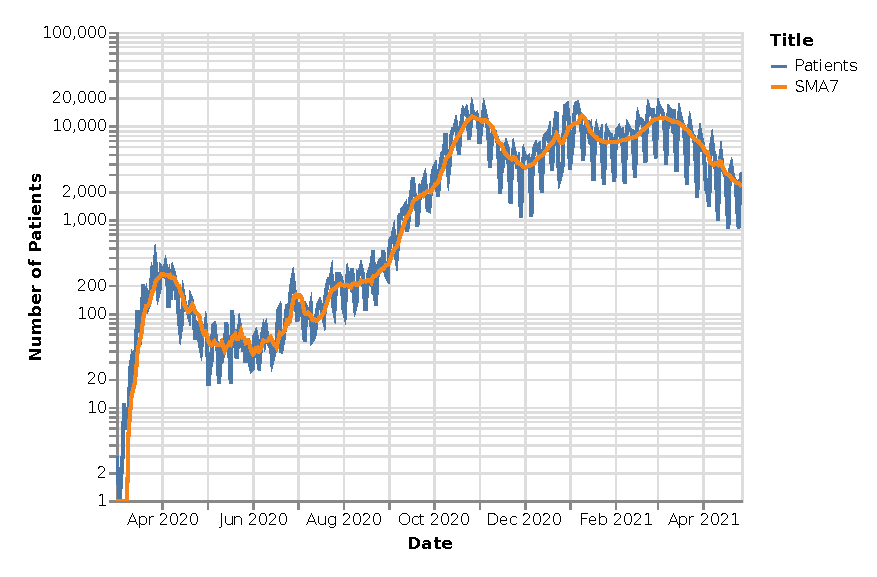
\includegraphics[width=0.9\textwidth]{figures/recovered-sma7.eps}
    \caption{Daily confirmed cases of infection and weekly moving average.}
    \label{fig:recovered-sma7}
\end{figure}
\FloatBarrier

\section{Summary}

The possibilities of analysis of the selected data set are limited and determining their quality is very difficult.
The main reason for the difficulties is the nature of the data, which corresponds in structure to econometric data, already processed in a certain way.
Thus, an available data catalog is in practice a set of results without background data.
Moreover, we tried to draw conclusions from existing data and tried to learn their quality without knowledge of the criterial limitations and general description of the data, which should be determined by the methodological guideline.
However, the instructions providing the necessary information about the data is missing (or is insufficiently informative) in these cases.

    \chapter{Conclusion and future work}\label{ch:conclusion-and-future-work}

\section{Future work}\label{sec:future-work}

We opened many topics in the paper but were unable to explore them in depth.
There are numerous ways in which the paper could be improved.

One topic that deserves more attention is the issue of data quality in relation to security constraints.
As discussed in Section~\ref{sec:data-quality-and-security}, data security and anonymization algorithms have an impact on data quality.
It would be interesting to measure the influence of these algorithms and compare them to reports on unclassified data in future work.

The use of quantitative methods for evaluating the quality of datasets is the second topic that was not sufficiently researched in the work.
Quantitative dimensions of quality were partially examined in the Section~\ref{sec:data-quality-dimensions}.
These dimensions were even put to the test on a portion of the data catalog.
However, the approach proved to be a dead end during the writing of the work because we couldn't objectively assess the current state of quality of the data catalog based on the measured values.

\section{Conclusion}\label{sec:conclusion}

The subject of data quality is extremely broad and diverse.
Although it may appear to be sufficiently researched at first glance, the application of specific (often very abstract) methodologies proves to be very problematic in practice.
It is necessary to ensure a~certain level of data source quality.
Whether it is for the needs of the company's management or for the needs of a machine learning algorithm.

The first contribution of this work is the definition of a new methodology for evaluating the quality of datasets, as well as the presentation of its application on three examples across the data centralization spectrum.
The second and most important contribution of this work is the evaluation of the catalog's quality using COVID-19 data from the Institute of Health Information and Statistics of the Czech Republic.
The analysis was evaluated within the framework of the methodology that we defined.

We attempted an objective evaluation of the data catalog.
However, because a~portion of the questionnaire used could not be answered, a correction by a specialist in the field would be appropriate.
This, however, does not diminish the importance of our work, which can now serve as a standard against which future work can be measured.
It is critical to perform repeated evaluations in order to gradually improve data quality.
However, due to the time consuming nature of such work, part of the process would need to be automated.


    \begin{appendices}
        \chapter{Data Quality Attributes}\label{ch:data-quality-attributes}

Eppler (2006) presented list of seventy of the most used data and information quality criteria explicitly defined in the literature.
They provide the basis for most of the DQ frameworks.

\begin{figure}[htb]
    \footnotesize

    \begin{multicols}{3}
        \begin{enumerate}
            \item Comprehensiveness
            \item Accuracy
            \item Clarity
            \item Applicability
            \item Conciseness
            \item Consistency
            \item Correctness
            \item Currency
            \item Convenience
            \item Timeliness
            \item Traceability
            \item Interactivity
            \item Accessibility
            \item Security
            \item Maintainability
            \item Speed
            \item Objectivity
            \item Attributability
            \item Value-added
            \item Reputation (source)
            \item Ease-of-use
            \item Precision
            \item Comprehensibility
            \item Trustworthiness\newline (source)
            \item Reliability
            \item Price 
            \item Verifiability
            \item Testability
            \item Provability
            \item Performance
            \item Ethics
            \item Privacy
            \item Helpfulness
            \item Neutrality
            \item Ease of Manipulation
            \item Validity
            \item Relevance
            \item Coherence
            \item Interpretability
            \item Completeness
            \item Learnability
            \item Exclusivity
            \item Right Amount
            \item Existence of meta information
            \item Appropriateness\newline of meta information
            \item Target group orientation
            \item Reduction of complexity
            \item Response time
            \item Believability
            \item Availability
            \item Consistent Representation
            \item Ability to represent null values
            \item Semantic Consistency
            \item Concise Representation
            \item Obtainability
            \item Stimulating
            \item Attribute granularity
            \item Flexibility
            \item Reflexivity
            \item Robustness
            \item Equivalence of redundant or distributed data
            \item Concurrency of redundant or distributed data
            \item Nonduplication
            \item Essentialness
            \item Rightness
            \item Usability
            \item Cost
            \item Ordering
            \item Browsing
            \item Error rate
        \end{enumerate}
    \end{multicols}

    \centering
    \caption{Data \& Information Quality Criteria~\cite{eppler2006}}
    \label{fig:dq-criteria}
\end{figure}
\FloatBarrier
    
        \chapter{Dataset Collection}\label{ch:dataset-collection}

\begin{table}[htbp]
    \centering

    \begin{longtable}{@{}rp{10cm}l@{}}
        \toprule
        \# & Title                                                                                                                                                               & Category                          \\ \midrule
         1 & Základní přehled                                                                                                                                                    & Epidemiologické charakteristiky   \\
         2 & Přehled osob s prokázanou nákazou dle hlášení krajských hygienických stanic (v2)                                                                                    & Epidemiologické charakteristiky   \\
         3 & Celkový (kumulativní) počet osob s prokázanou nákazou dle krajských hygienických stanic včetně laboratoří (v2)                                                      & Epidemiologické charakteristiky   \\
         4 & Přehled vyléčených dle hlášení krajských hygienických stanic                                                                                                        & Epidemiologické charakteristiky   \\
         5 & Přehled úmrtí dle hlášení krajských hygienických stanic                                                                                                             & Epidemiologické charakteristiky   \\
         6 & Přehled hospitalizací                                                                                                                                               & Epidemiologické charakteristiky   \\
         7 & Celkový (kumulativní) počet osob s prokázanou nákazou dle krajských hygienických stanic včetně laboratoří, počet vyléčených, počet úmrtí a provedených testů (v2)   & Epidemiologické charakteristiky   \\
         8 & Přehled epidemiologické situace dle hlášení krajských hygienických stanic podle okresu                                                                              & Epidemiologické charakteristiky   \\
         9 & Přehled epidemiologické situace dle hlášení krajských hygienických stanic podle ORP                                                                                 & Epidemiologické charakteristiky   \\
        10 & Epidemiologická charakteristika obcí                                                                                                                                & Epidemiologické charakteristiky   \\
        11 & Epidemiologická charakteristika městských částí hlavního města Prahy                                                                                                & Epidemiologické charakteristiky   \\
        12 & Celkový (kumulativní) počet provedených testů (v2)                                                                                                                  & Testování                         \\
        13 & Přehled provedených testů podle typu a indikace                                                                                                                     & Testování                         \\
        14 & Celkový (kumulativní) počet provedených testů podle krajů a okresů ČR                                                                                               & Testování                         \\
        15 & Odběrová místa v ČR                                                                                                                                                 & Testování                         \\
        16 & Přehled vykázaných očkování podle krajů ČR                                                                                                                          & Očkování                          \\
        17 & Přehled vykázaných očkování podle očkovacích míst ČR                                                                                                                & Očkování                          \\
        18 & Očkovací místa v ČR                                                                                                                                                 & Očkování                          \\
        19 & Přehled spotřeby podle očkovacích míst ČR                                                                                                                           & Očkování                          \\
        20 & Přehled distribuce očkovacích látek v ČR                                                                                                                            & Očkování                          \\
        21 & Přehled registrací podle očkovacích míst ČR                                                                                                                         & Očkování                          \\
        22 & Přehled rezervací podle očkovacích míst ČR                                                                                                                          & Očkování                          \\
        23 & Přehled vykázaných očkování podle profesí                                                                                                                           & Očkování                          \\
        24 & Přehled distribuce ochranného materiálu dle krajů ČR (v2)                                                                                                           & Různé                             \\
        \bottomrule
    \end{longtable}

    \caption{Available datasets and their categories with original, Czech titles}
    \label{table:available-datasets}
\end{table}

        \chapter{Metadata File Structure}\label{ch:metadata-file-structure}

\begin{figure}[htb]
    \centering
    \begin{lstlisting}[language=json,firstnumber=1]
{
    "@context": [
        "http://www.w3.org/ns/csvw",
        {
            "@language": "cs"
        }
    ],
    "url": "zakladni-prehled.csv",
    "dc:title": "COVID-19: Zakladni prehled",
    "dc:description": "...",
    "dc:source": "Krajske hygienicke stanice v CR",
    "dcat:keyword": ["COVID-19", "widget", "aktualni situace"],
    "dc:publisher": {
        "schema:name": "UZIS CR",
        "schema:url": {
            "@id": "https://www.uzis.cz/"
        }
    },
    "dc:license": {
        "@id": "https://data.gov.cz/podminky-uziti/volny-pristup/"
    },
    "dc:modified": {
        "@value": "2021-04-18",
        "@type": "xsd:date"
    },
    "tableSchema": {
        "columns": [
            {
                "name": "datum",
                "titles": "datum",
                "datatype": "date",
                "dc:description": "Datum vytvoreni aktualizace."
            },...
        ]
    }
}
    \end{lstlisting}

    \caption{Metadata file structure}
    \label{ls:metadata}
\end{figure}
\FloatBarrier

        % \definecolor{codegreen}{rgb}{0,0.6,0}
\definecolor{codegray}{rgb}{0.5,0.5,0.5}
\definecolor{codepurple}{rgb}{0.58,0,0.82}

\lstdefinestyle{mystyle}{
    commentstyle=\color{codegreen},
    keywordstyle=\color{magenta},
    numberstyle=\tiny\color{codegray},
    stringstyle=\color{codepurple},
    basicstyle=\footnotesize,
    breakatwhitespace=false,
    breaklines=true,
    captionpos=b,
    keepspaces=true,
    numbers=left,
    numbersep=5pt,
    showspaces=false,
    showstringspaces=false,
    showtabs=false,
    tabsize=2
}

\lstset{style=mystyle}

\chapter{URL tokenizer}\label{ch:url-tokenizer}

Implementation of algorithm infering the location of spaces in a~string as presented in the original \textit{StackOverflow} question~\cite{stackoverflow:tokenizer}.
The code is written at the Python programming language.

\begin{lstlisting}[language=Python]
    from math import log

    words = open("words-by-frequency.txt").read().split()
    wordcost = dict((k, log((i+1)*log(len(words)))) for i,k in enumerate(words))
    maxword = max(len(x) for x in words)


    def infer_spaces(s):

        def best_match(i):
            candidates = enumerate(reversed(cost[max(0, i-maxword):i]))
            return min((c + wordcost.get(s[i-k-1:i], 9e999), k+1) for k,c in candidates)

        # Build the cost array.
        cost = [0]
        for i in range(1,len(s)+1):
            c,k = best_match(i)
            cost.append(c)

        # Backtrack to recover the minimal-cost string.
        out = []
        i = len(s)
        while i>0:
            c,k = best_match(i)
            assert c == cost[i]
            out.append(s[i-k:i])
            i -= k

        return " ".join(reversed(out))
\end{lstlisting}

        % \chapter{Sources}\label{ch:sources}

\section{Source Code}\label{sec:source-code}

Source code used in the thesis is available at \url{https://github.com/mareklovci/dip-code}.

\section{Source \LaTeX}\label{sec:source-latex}

Source code for thesis text is available at \url{https://github.com/mareklovci/dip-paper}

    \end{appendices}

    %\newpage
    %\printglossary[type=\acronymtype]
    %\printglossary

    \newpage
    \printbibliography

\end{document}
